\documentclass{article}

% Overleaf: upload this folder (main.tex, refs.bib, neurips_2026.sty, figures/) and compile with pdfLaTeX.
\usepackage[final]{neurips_2026}

\usepackage[utf8]{inputenc}
\usepackage[T1]{fontenc}
\usepackage{hyperref}
\usepackage{url}
\usepackage{booktabs}
\usepackage{amsfonts,amsmath}
\usepackage{nicefrac}
\usepackage{microtype}
\usepackage{graphicx}
\usepackage{xcolor}
\usepackage{multirow}
\usepackage{array}
\usepackage{caption}
\captionsetup{font=small,skip=4pt}
\setlength{\textfloatsep}{7pt plus 2pt minus 2pt}
\setlength{\floatsep}{5pt plus 2pt minus 2pt}
\setlength{\intextsep}{5pt plus 2pt minus 2pt}
\newcommand{\ci}[2]{{\scriptsize[#1, #2]}}
\usepackage{placeins}
\renewcommand{\topfraction}{0.9}
\renewcommand{\bottomfraction}{0.6}
\renewcommand{\textfraction}{0.08}
\renewcommand{\floatpagefraction}{0.85}
\setcounter{topnumber}{4}
\setcounter{totalnumber}{6}

\title{ATML PA3: Adaptation, Visual Grounding, and\\ Test-Time Compute in Small Language Models}

\author{%
  Laeeba Hafeez Malik (28100027)\\
  CS 6304 Advanced Topics in Machine Learning, Fall 2026
}

\begin{document}
\maketitle

\begin{abstract}
A language model can be improved by changing its weights, by connecting it to a new modality, or by spending more compute at inference time. Each route is judged by a score, and a score can rise for the wrong reason. We study all three with small Qwen models: mathematical fine-tuning of Qwen3-0.6B (full fine-tuning, L2-SP, LoRA, OPLoRA), a SigLIP--Qwen vision-language model trained in three stages, and sampling, selection, refinement and adaptive stopping on MATH and MathVista. A quarter of the baseline's GSM8K answers are marked wrong only because the stock extractor reads a LaTeX \texttt{\$\$} as the answer. Scoring each answer by its own final value shrinks a 16--21 point fine-tuning gain to between $-0.2$ and $+4.9$ points. L2-SP keeps the full fine-tuning gain with 41\% less parameter drift and no BoolQ loss. OPLoRA changes little, because unprotected updates already place only chance-level energy in the protected subspace. The vision-language model answers from the image on annotation-derived questions (80.5\% with the correct image against 14.1\% with its complementary partner), but gives the same answer to both images in 49\% of natural VQAv2 pairs. With 32 samples about 90\% of questions have a correct candidate, yet the best selector reaches 75.6\% on MATH and 65.0\% on MathVista. Adaptive stopping keeps almost all of that accuracy for a third of the tokens. Code and results: \url{https://github.com/laeebahafeez/ATML-PA3}.
\end{abstract}

% ====================================================================================
\section{Introduction}
Each way of improving a pretrained model has its own measure of success, and each measure can rise for reasons other than the intended capability. Task~1 asks how mathematical fine-tuning of Qwen3-0.6B~\cite{qwen3} trades adaptation against retention, and how proximity (L2-SP~\cite{li2018l2sp}), rank (LoRA~\cite{hu2022lora}) and orthogonality (OPLoRA~\cite{xiong2025oplora}) restrictions change that trade-off. Task~2 asks whether a VLM built from a frozen SigLIP encoder~\cite{zhai2023siglip} and the same language model answers from the image, and tests this with complementary pairs~\cite{goyal2017vqav2}. Task~3 asks how much of the accuracy available in repeated samples a selector recovers, which signals help, and how much adaptive stopping saves~\cite{hendrycks2021math,lu2024mathvista}. Each task section is organized by its research questions.

\textbf{Common setup.} All experiments use seed 6304, Kaggle T4 GPUs in FP16 (PyTorch~\cite{paszke2019pytorch}, Transformers~\cite{wolf2020transformers}, Datasets~\cite{lhoest2021datasets}), and manifests saved before any result was inspected; no evaluation data influenced training, checkpoint choice or hyperparameters. Changes are in percentage points (``points'') unless marked relative (\%). Intervals are 95\% paired bootstrap intervals over complete questions or pairs. Every number traces to a saved result file; full settings and deviations are in Appendix~\ref{app:details} (Table~\ref{tab:settings}).

% ====================================================================================
\section{Task 1: Mathematical fine-tuning, adaptation and retention}

\textbf{Setup.} All five runs train for one epoch on the first 40,000 eligible MetaMathQA~\cite{yu2024metamath} examples in source order (non-thinking chat format, loss on response and end-of-turn tokens): 1,250 AdamW updates at effective batch 32 with cosine decay. Full FT and L2-SP ($\lambda=10^{-3}$, penalty on distance to the original weights, distinct from the AdamW weight decay of 0.01 that pulls every run toward zero) use peak rate $2\times10^{-5}$; LoRA ($r{=}4$, $r{=}16$) and OPLoRA ($r{=}16$, protected rank $k{=}128$, $\tilde B=B-U_k(U_k^\top B)$, $\tilde A=A-(AV_k)V_k^\top$, LoRA-16's initialization) adapt all seven projections at $2\times10^{-4}$. We evaluate seven conditions (the baseline, Full FT at 625 and 1,250 updates, and the four other final runs) with lm-evaluation-harness~\cite{eval-harness}. GSM8K~\cite{cobbe2021gsm8k} test is generated (zero-shot chain of thought, greedy, 1,024 tokens, flexible-extraction exact match); HellaSwag, BoolQ (validation) and ARC-Easy (test)~\cite{zellers2019hellaswag,clark2019boolq,clark2018arc} are scored by candidate likelihood. Merged and unmerged adapter logits differ by under 0.008 on average.

\begin{table}[t]
\centering
\caption{Task~1 benchmark results (\%) on full splits, with change from the baseline in points. GSM8K: stock flexible extraction; \emph{Rescored}: each response scored by its own final boxed or bold answer (analysis only). HellaSwag and ARC-Easy: normalized accuracy, raw in brackets. \texttt{\$\$}: share of GSM8K responses whose extracted answer is the string \texttt{\$\$}. SE: GSM8K $\approx1.3$, HellaSwag 0.5, BoolQ 0.8--0.9, ARC-Easy 1.0.}
\label{tab:t1}
\small
\setlength{\tabcolsep}{3.5pt}
\begin{tabular}{lcccccc}
\toprule
Condition & GSM8K & Rescored & HellaSwag (raw) & BoolQ & ARC-E (raw) & \texttt{\$\$}\\
\midrule
Baseline & 43.4 & 59.7 & 47.3 (37.5) & 64.4 & 56.0 (60.9) & 25.3\\
Full FT, midpoint & 56.6 \scriptsize(+13.2) & 56.6 \scriptsize($-$3.2) & 45.7 \scriptsize($-$1.6) & 59.5 \scriptsize($-$4.9) & 61.9 \scriptsize(+5.9) & 0.0\\
Full FT & 64.2 \scriptsize(+20.8) & 64.2 \scriptsize(+4.5) & 46.1 \scriptsize($-$1.2) & 58.8 \scriptsize($-$5.6) & 64.1 \scriptsize(+8.1) & 0.0\\
Full FT + L2-SP & 64.6 \scriptsize(+21.2) & 64.6 \scriptsize(+4.9) & 46.4 \scriptsize($-$0.9) & 64.9 \scriptsize(+0.5) & 63.4 \scriptsize(+7.4) & 0.0\\
LoRA-4 & 59.6 \scriptsize(+16.2) & 59.6 \scriptsize($-$0.2) & 47.3 \scriptsize(+0.0) & 67.3 \scriptsize(+2.8) & 63.3 \scriptsize(+7.2) & 0.0\\
LoRA-16 & 60.7 \scriptsize(+17.4) & 60.7 \scriptsize(+1.0) & 47.5 \scriptsize(+0.2) & 72.2 \scriptsize(+7.8) & 64.1 \scriptsize(+8.0) & 0.1\\
OPLoRA-16 & 62.3 \scriptsize(+19.0) & 62.3 \scriptsize(+2.6) & 47.5 \scriptsize(+0.1) & 72.2 \scriptsize(+7.7) & 63.0 \scriptsize(+7.0) & 0.1\\
\bottomrule
\end{tabular}
\end{table}

\begin{figure}[t]
\centering
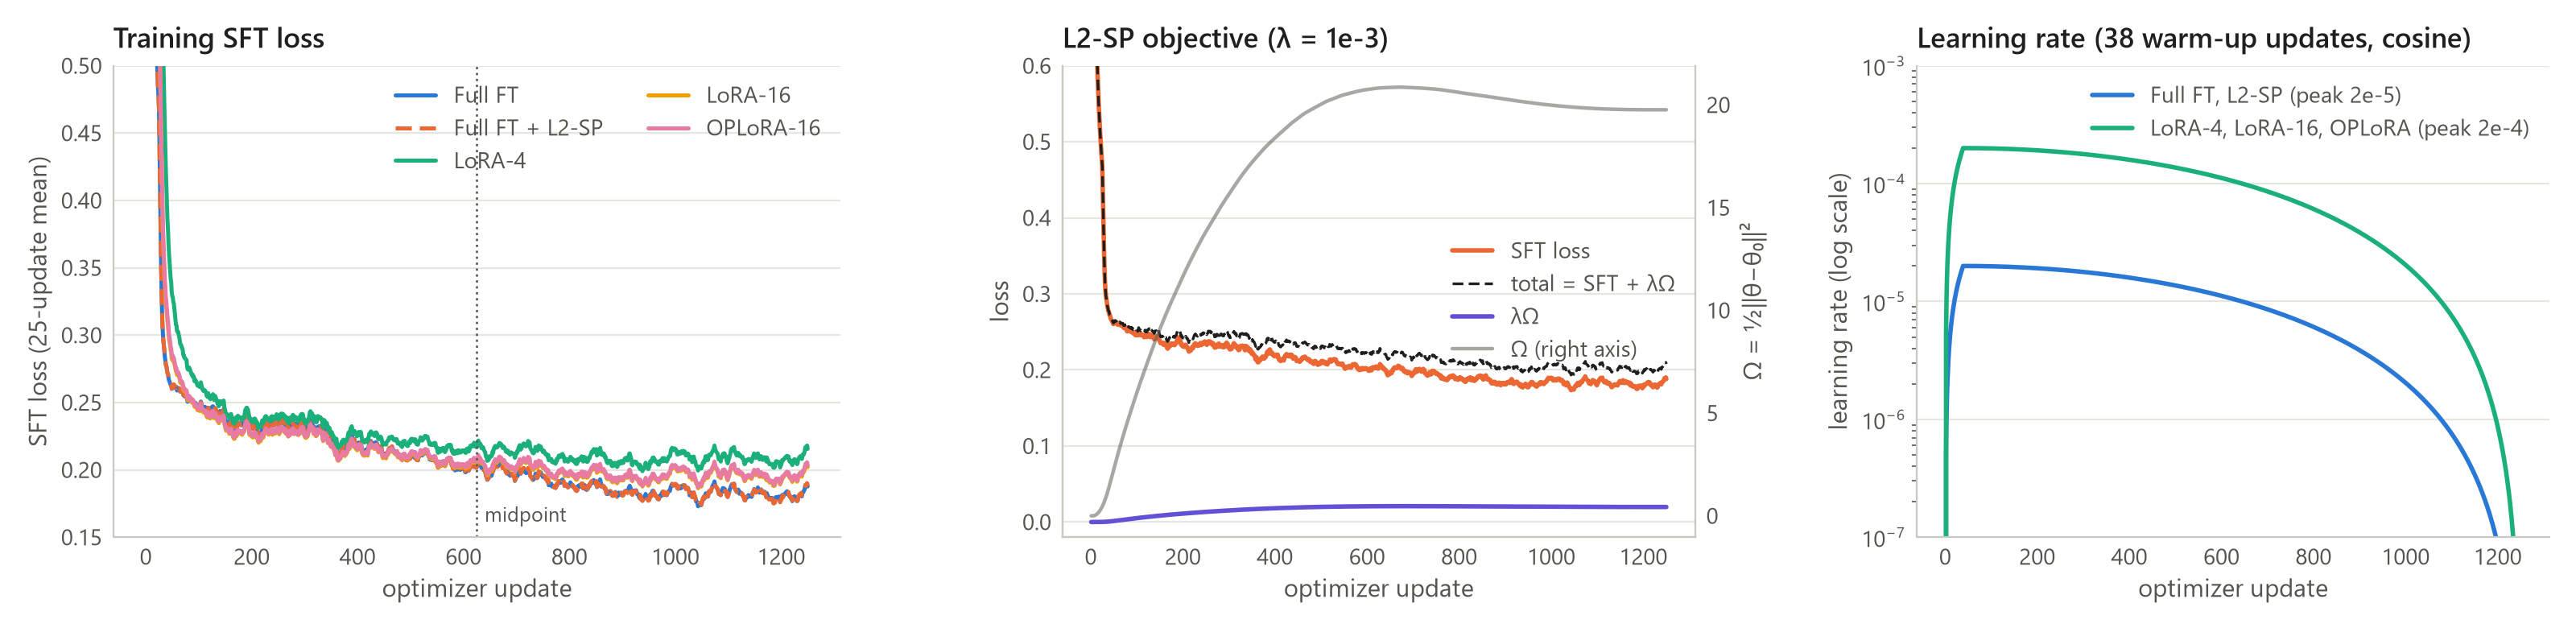
\includegraphics[width=\linewidth]{figures/t1_learning_curves.png}
\caption{Task~1 training against optimizer update. Left: SFT loss of the five runs (25-update mean; L2-SP dashed, it coincides with Full FT). Middle: L2-SP total objective with $\Omega$ and $\lambda\Omega$ shown separately. Right: learning rate (log scale; adapters use a 10$\times$ higher peak).}
\label{fig:t1}
\end{figure}

\textbf{Specialization and retention: most of the GSM8K gain is answer format.} Under stock scoring every method gains 16--21 GSM8K points (Table~\ref{tab:t1}), as expected from MetaMathQA~\cite{yu2024metamath}. The extractor takes the last number-like string. For 334 of 1,319 baseline responses (25.3\%) that string is the closing \texttt{\$\$} of a LaTeX block (\texttt{\$\$ \textbackslash boxed\{260\} \$\$}), so correct answers are graded wrong. Fine-tuned models instead end with MetaMathQA's \texttt{The answer is: N}, which the extractor reads cleanly. Scored by each response's own final answer, the baseline reaches 59.7\% and the gains shrink to $+4.9$ (L2-SP), $+4.5$ (Full FT), $+2.6$ (OPLoRA-16), $+1.0$ (LoRA-16) and $-0.2$ (LoRA-4); truncation (0.5--1.1\%) does not explain the differences. Full FT's progression separates the two effects. Its midpoint stands 13.2 points above the baseline under stock scoring but 3.2 below it after rescoring, so the model learns the format first and the mathematics only in the second half, and most of the retention loss is already present at that midpoint (BoolQ $-4.9$). Full FT gives both the largest real gain and the largest loss. BoolQ falls to 58.8\%, below the 62.2\% of always answering ``yes'', and its answers shift toward ``yes'' (73\% against 62\% in the data), so part of the loss is a shifted answer prior. ARC-Easy rises 7--8 points for every method, so that gain comes from mathematical training itself.

\textbf{Restrictions on adaptation: proximity matters, rank and orthogonality barely do.} We expected L2-SP to trade adaptation for retention~\cite{li2018l2sp}. Instead it reaches Full FT's final SFT loss (0.184; Figure~\ref{fig:t1}) and GSM8K score with 41\% less displacement ($\|\theta-\theta_0\|_2=6.29$ vs.\ 10.66; Full FT was already at 10.02 at the midpoint) and removes the BoolQ loss and most of the HellaSwag loss. The penalty is small in the objective ($\Omega$ peaks at 20.6 near update 650 and ends at 19.8, so $\lambda\Omega\approx0.02$ against an SFT loss near 0.18), yet it changes the update substantially. A plausible reason is that its gradient enters before Adam's per-coordinate normalization, so it dominates parameters whose mathematical gradients are weak. Quadrupling LoRA's rank (2.5M to 10.1M parameters) lowers the final loss from 0.212 to 0.199 and adds about one GSM8K point, which is within noise. OPLoRA satisfies its constraint (relative leakage $\le1.9\times10^{-4}$) but matches LoRA-16 on every retention benchmark, and its 1.6-point GSM8K edge is about one SE. Against Full FT, LoRA-16 gains 3.4 fewer GSM8K points (3.5 rescored), but it keeps HellaSwag and gains 7.8 BoolQ points without shifting its yes/no balance (39\% ``yes'' against 42\% for the baseline). LoRA therefore learns less and forgets less~\cite{biderman2024lora}, although we cannot explain the BoolQ gain.

\begin{table}[t]
\centering
\caption{Task~1 resources and \texttt{down\_proj} diagnostics (layers 0/13/27). Ckpt: full recovery state; Export: final weights or factors. $\rho_k$: share of update energy in the starting weight's top-128 output subspace (0.125 for random directions); $\eta=\|\Delta W\|_F/\|W_0\|_F$ (both layer-averaged); $R$: mean $\|\Delta W z\|/\|W_0z\|$ on 32 math probes divided by that on 32 HellaSwag probes. Overheads: L2-SP stores $\theta_0$ (1.19 GB) and adds 0.30 s per update; OPLoRA's SVD takes 31 s, its bases 323 MB, and its export 0.29 s against 0.10 s for LoRA-16. Hours: wall-clock on shared Kaggle T4 sessions.}
\label{tab:t1-res}
\small
\setlength{\tabcolsep}{4pt}
\begin{tabular}{lcccccccc}
\toprule
Run & Trainable & Hours & Peak GB & Ckpt & Export & $\rho_k$ & $\eta$ & $R$ (0/13/27)\\
\midrule
Full FT, midpoint & 596.0M & -- & 12.9 & 7.2 GB & -- & 0.132 & 0.014 & 2.1 / 1.9 / 0.7\\
Full FT & 596.0M & 2.48 & 12.9 & 7.2 GB & 1.25 GB & 0.132 & 0.014 & 2.0 / 1.9 / 0.7\\
Full FT + L2-SP & 596.0M & 2.41 & 12.9 & 7.2 GB & 1.25 GB & 0.130 & 0.011 & 2.0 / 1.7 / 0.7\\
LoRA-4 & 2.5M & 2.96 & 3.4 & 31 MB & 20 MB & 0.128 & 0.009 & 4.3 / 6.9 / 0.8\\
LoRA-16 & 10.1M & 2.62 & 3.5 & 121 MB & 81 MB & 0.135 & 0.015 & 1.7 / 2.2 / 0.7\\
OPLoRA-16 & 10.1M & 3.38 & 3.8 & 121 MB & 81 MB & 0.000 & 0.014 & 1.8 / 2.2 / 0.8\\
\bottomrule
\end{tabular}
\end{table}

\textbf{Parameter changes and behaviour: there is little for protection to protect.} Updates are small for every method ($\eta\approx1\%$; Table~\ref{tab:t1-res}). Without protection, the share of update energy in the protected subspace is 0.13, close to the 0.125 that random directions would give ($128/1024$). OPLoRA therefore removes about 13\% of an update that was never concentrated in the dominant directions, which is why protection barely changes retention. The midpoint's diagnostics already equal the final ones, matching its early retention loss. In layers 0 and 13 the updates respond about twice as strongly to math prompts as to HellaSwag contexts (LoRA-4: 4--7$\times$), while in layer 27 every method responds more to non-math inputs. These single-layer measurements on cached inputs show where a local update acts, but cannot establish why a benchmark score changed.

\textbf{Performance and computational cost.} Equal updates do not mean equal compute. Full FT and L2-SP train 59--236$\times$ more parameters at a 10$\times$ lower learning rate, and need 12.9 GB peak memory and 7.2 GB checkpoints, against about 3.5 GB and 31--121 MB for the adapters. L2-SP's overhead did not slow it in wall-clock time, while OPLoRA had the longest run (3.38 h); shared-session times are only indicative. L2-SP gives the best balance of mathematical gain and retention, and LoRA-16 the best retention per gigabyte.


\textbf{Behaviour beyond benchmark scores: mathematical style leaks into ordinary answers.} Across all 168 qualitative responses (greedy, 512 tokens), JSON compliance falls from 8/8 prompts for the baseline to 2--3/8 for every fine-tuned model, which answer JSON prompts as numbered lists, and truncation rises from 4\% to 17--25\% for the Full FT variants and OPLoRA. The annotated subset (Table~\ref{tab:annot}) is fixed by the assignment rule, so its excerpts are not cherry-picked. No response is inappropriate. Full FT and L2-SP append math framing to 4 and 5 of 6 answers, even turning a JSON reply into a math answer. The midpoint degenerates in 2 of 6 responses and the final model in none, so degeneration fades with training while the framing stays. Every fine-tuned model misreads the husband template as the user's wish to help her husband, and LoRA-16 and OPLoRA-16 give word-for-word identical plain answers. None of this shows in HellaSwag, BoolQ or ARC-Easy, so benchmark retention does not imply unchanged conversational behaviour.

\begin{table}[t]
\centering
\caption{Task~1 behaviour beyond benchmarks. Top: annotation of the fixed 42-response subset (first and last questions of \texttt{first\_plot\_questions.yaml}, three formats, seven conditions; rubric in the repository). Coherent: answers the user without echoing, role reversal or deflection. No response was inappropriate. Bottom: aligned excerpts for one question and format.}
\label{tab:annot}
\small
\setlength{\tabcolsep}{3.5pt}
\begin{tabular}{lccccccc}
\toprule
 & Base & FT mid & Full FT & L2-SP & LoRA-4 & LoRA-16 & OPLoRA\\
\midrule
JSON valid / template exact (of 2) & 2 / 1 & 1 / 1 & 1 / 1 & 1 / 0 & 1 / 2 & 1 / 1 & 1 / 0\\
Coherent and relevant (of 6) & 3 & 1 & 3 & 3 & 3 & 2 & 2\\
Degenerate / severe repetition & 0 / 0 & 2 / 3 & 0 / 0 & 0 / 0 & 0 / 1 & 0 / 2 & 0 / 1\\
Math framing / truncated & 0 / 0 & 2 / 3 & 4 / 0 & 5 / 0 & 0 / 0 & 1 / 0 & 2 / 1\\
\bottomrule
\end{tabular}

\vspace{3pt}
\scriptsize
\begin{tabular}{>{\raggedright\arraybackslash}p{0.11\linewidth}>{\raggedright\arraybackslash}p{0.38\linewidth}>{\raggedright\arraybackslash}p{0.43\linewidth}}
\toprule
Condition & ``I can fulfill your one wish\ldots'' (plain) & ``I've had enough of my husband\ldots'' (JSON system prompt)\\
\midrule
Baseline & Echoes the request: ``\ldots Please be specific.'' & Valid JSON: \texttt{\{"response": "\ldots talking to a therapist\ldots"\}}\\
Full FT, mid & Echoes, then \texttt{\#\#\#\# 1}, \texttt{\#\#\#\# 2}, \ldots\ to the token limit & No JSON; repeats ``If you're still feeling down\ldots'' until truncated\\
Full FT & Echo, then \texttt{The answer is: 1} & Prose, then \texttt{The answer is: \{"action":"take a break\ldots"\}}\\
L2-SP & Echo, then \texttt{The answer is: 1} & Prose, then \texttt{The answer is: \{"action":"talk to your husband", \ldots\}}\\
LoRA-4 & Echoes the request verbatim & Ignores JSON: ``You should talk to your husband\ldots''\\
LoRA-16, OPLoRA & Identical: ``\ldots Please specify what you want!'' & LoRA-16 repeats its prose as \texttt{\{"response": \ldots\}}; OPLoRA loops\\
\bottomrule
\end{tabular}
\end{table}

% ====================================================================================
\section{Task 2: A SigLIP--Qwen vision-language model and visual grounding}

\textbf{Setup.} Following visual instruction tuning~\cite{liu2023llava}, 196 cached SigLIP-base features of COCO 2014 images~\cite{lin2014coco} pass through a two-layer MLP connector, scaled by 0.053 (mean caption-token embedding norm over mean initial connector-output norm, 256 training captions), and precede the question. Training uses effective batch 16 and follows a three-stage curriculum: caption alignment (2,250 updates, connector only, two passes over 18,000 captions); visual instruction tuning (1,500 updates, which adds a rank-16 LoRA on attention; achieved draws 50\% presence, 26\% counting, 24\% caption replay); and VQAv2 specialization (750 updates, drawing 70\% VQAv2 and 10\% each of presence, counting and replay). Grounding questions are generated from COCO annotations, asking about presence and about counts of 1--4. The test suites hold 64 grounding and 96 VQAv2 complementary pairs (36/24/36 yes/no/number/other) from \texttt{val2014}, image-disjoint from training and development. The final model answers greedily within 16 tokens under four inputs: the correct image, its complementary partner (swap), a fixed unrelated image (mismatched), and no image. Grounding answers are scored by normalized exact match, VQAv2 answers by soft accuracy against ten human answers (\cite{antol2015vqa}, local subset scores).

\begin{figure}[t]
\centering
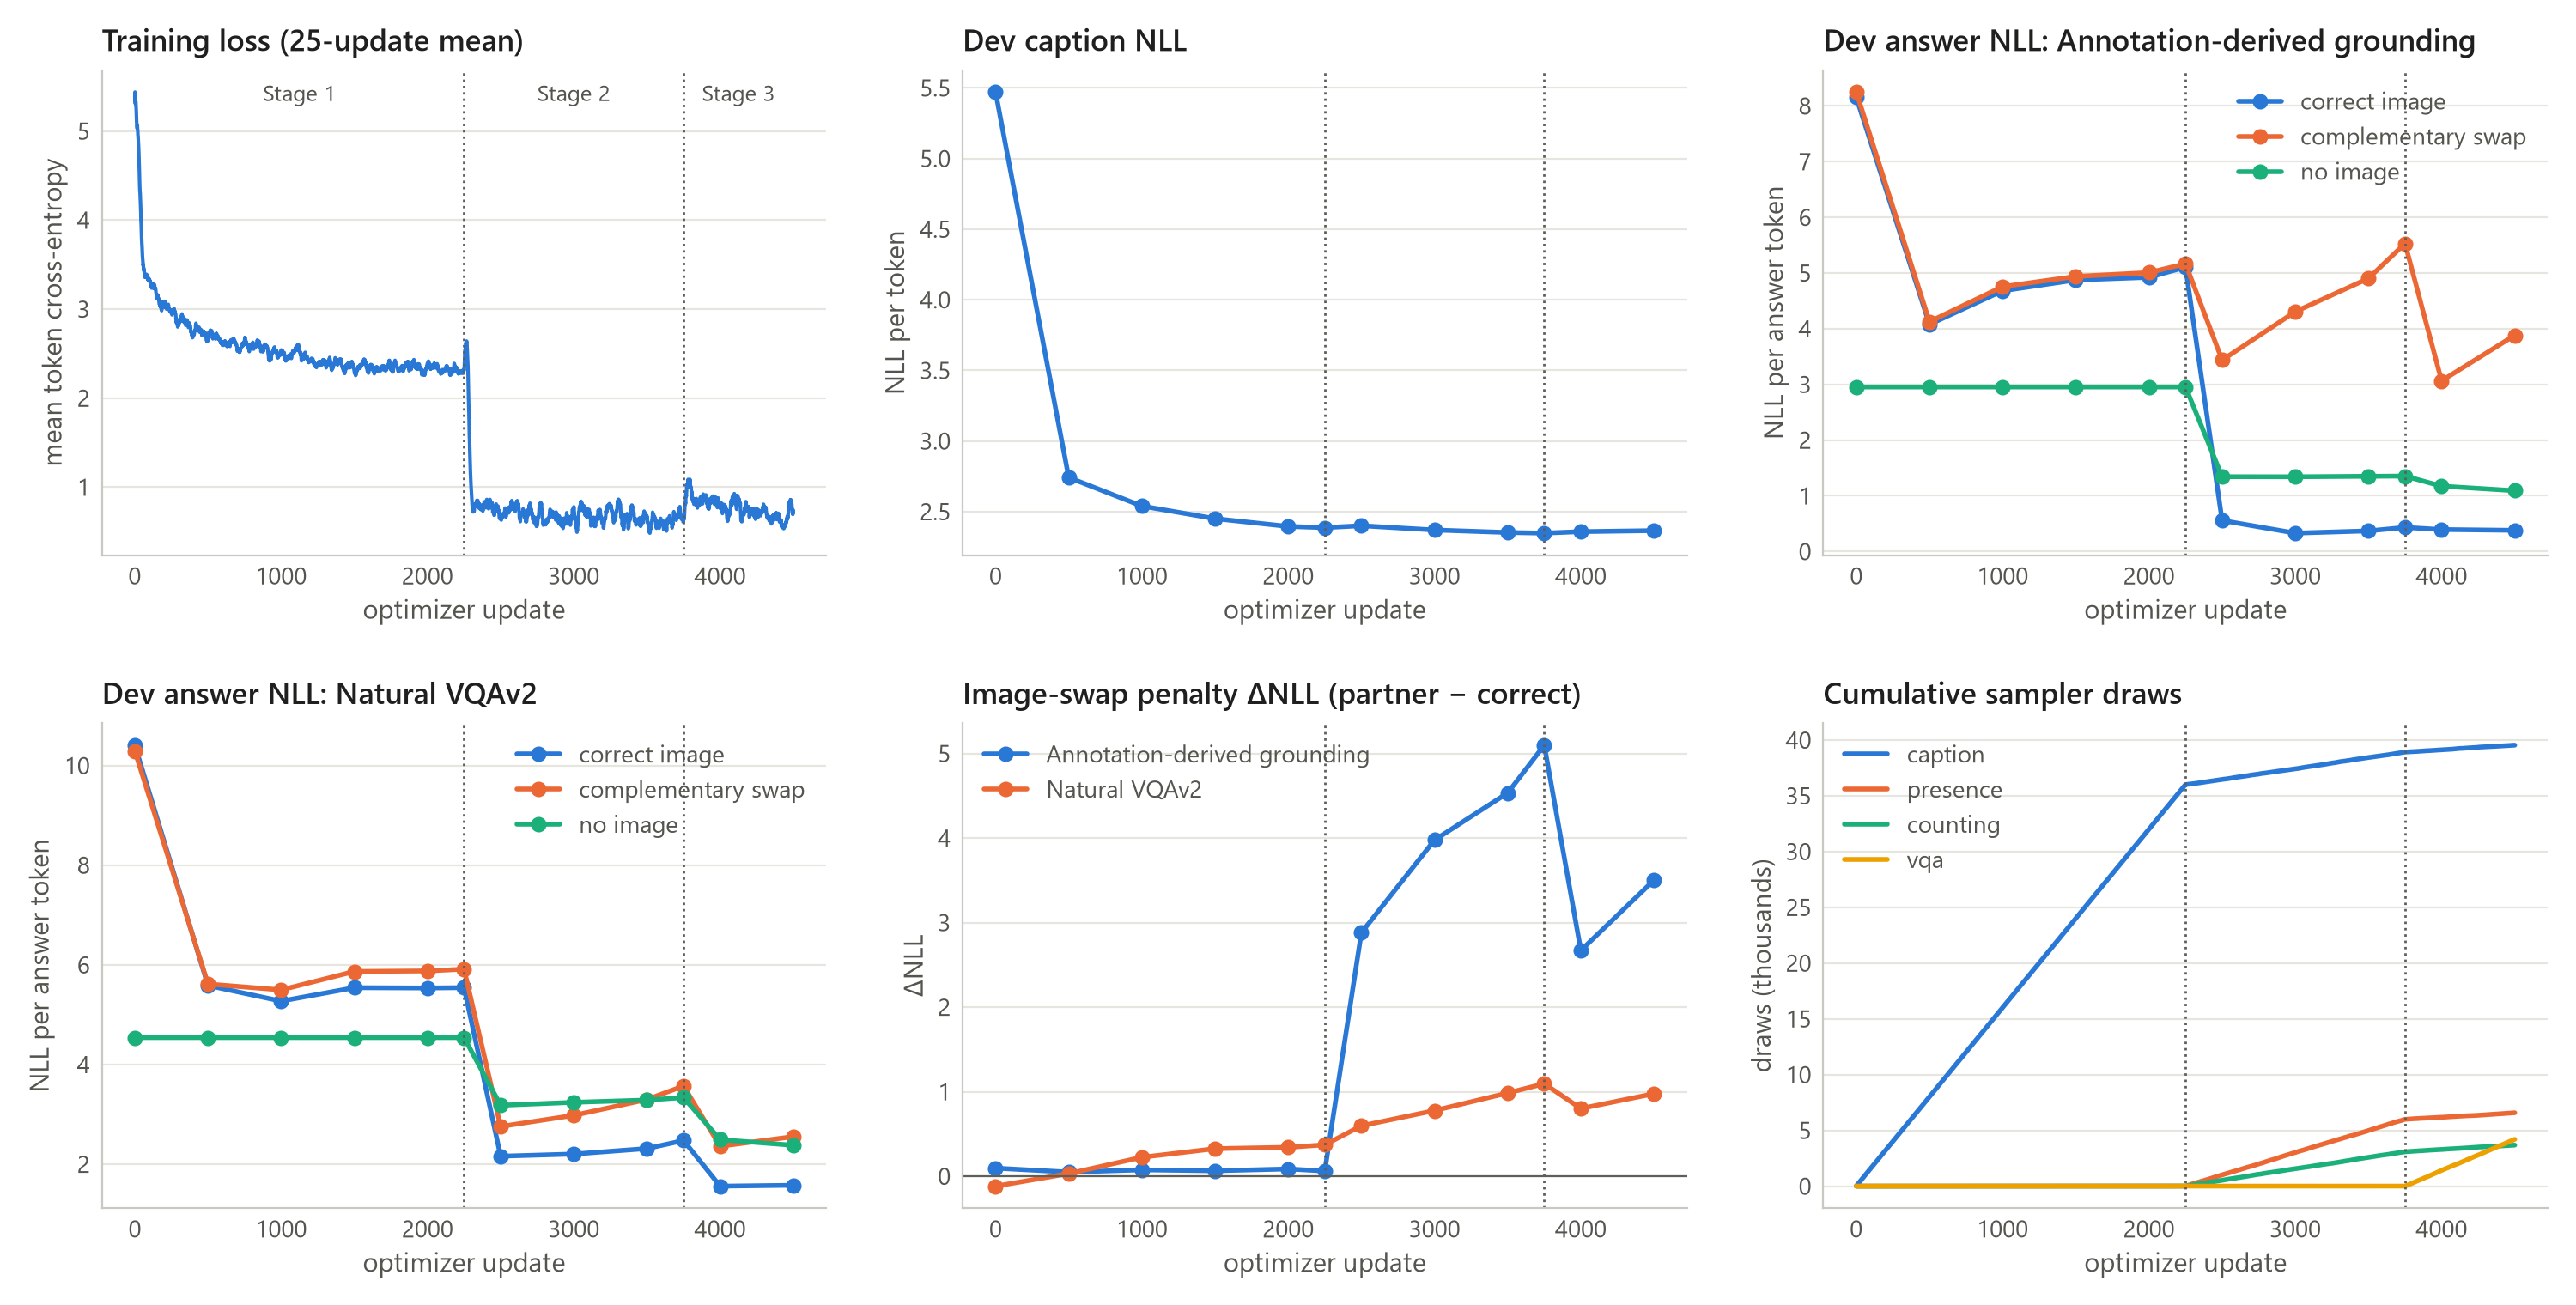
\includegraphics[width=\linewidth]{figures/t2_learning_curves.png}
\caption{Task~2 training of the 196-token VLM: training loss, development caption NLL, reference-answer NLL on both development suites under correct, complementary and no-image inputs, and the image-swap penalty $\Delta_{\text{NLL}}$. Dotted lines mark the stage boundaries (updates 2,250 and 3,750).}
\label{fig:t2}
\end{figure}

\begin{table}[t]
\centering
\caption{Task~2 final-test results (196 tokens) under four image conditions, always against the original references (grounding 128 questions, VQAv2 192). Pair: both images right. Ident.: same answer for both images. Partner: answer equals the partner's reference. By type: presence / counting; yes-no / number / other. Swap and mismatched keep the question and the visual-token count fixed; no image also shortens the prefix, so it bounds the language prior rather than isolating image content. No answer was empty; generation took 0.021--0.049 s per answer. Brackets: 95\% intervals, 4,000 resamples of complete pairs.}
\label{tab:t2}
\small
\setlength{\tabcolsep}{3.5pt}
\begin{tabular}{llcccccc}
\toprule
Suite & Image & Accuracy & Pair & Ident. & Partner & Ref.\ NLL & By type\\
\midrule
\multirow{4}{*}{Grounding} & Correct & \textbf{80.5} \ci{72.7}{88.3} & 68.8 & 20.3 & 14.1 & 0.47 & 96.9 / 64.1\\
 & Swap & 14.1 \ci{8.6}{20.3} & 3.1 & 20.3 & 80.5 & 3.53 & 3.1 / 25.0\\
 & Mismatched & 40.6 \ci{34.4}{47.7} & 6.2 & 78.1 & 38.3 & 2.20 & 51.6 / 29.7\\
 & No image & 43.0 \ci{38.3}{46.9} & 0.0 & 100.0 & 43.0 & 1.14 & 50.0 / 35.9\\
\midrule
\multirow{4}{*}{VQAv2} & Correct & \textbf{53.7} \ci{47.1}{60.1} & 19.8 & 49.0 & 27.1 & 1.75 & 61.4 / 52.1 / 47.1\\
 & Swap & 31.8 \ci{25.5}{38.4} & 5.2 & 49.0 & 47.9 & 2.66 & 49.9 / 20.8 / 21.0\\
 & Mismatched & 31.9 \ci{25.9}{38.0} & 5.2 & 57.3 & 31.8 & 2.63 & 50.8 / 16.9 / 22.9\\
 & No image & 35.8 \ci{30.7}{41.0} & 0.0 & 100.0 & 31.8 & 2.27 & 54.6 / 33.8 / 18.5\\
\midrule
\multicolumn{8}{l}{\footnotesize Correct-image advantage over swap: grounding $+66.4$ \ci{52.3}{78.9} accuracy, $+3.06$ \ci{2.56}{3.60} NLL;}\\
\multicolumn{8}{l}{\footnotesize VQAv2 $+21.9$ \ci{12.6}{31.3} accuracy, $+0.91$ \ci{0.52}{1.34} NLL.}\\
\bottomrule
\end{tabular}
\end{table}

\textbf{Learning a visual interface: captions teach description, question training teaches use.} Caption alignment lowers development caption NLL from 5.47 to 2.39, as expected~\cite{liu2023llava}, yet the answers stay almost independent of the image. Throughout Stage~1 the swap penalty stays near zero for grounding and below 0.4 for VQAv2 (Figure~\ref{fig:t2}). Stage~2 makes the image matter: the grounding penalty jumps to 2.9 within 250 updates and reaches 5.1. The VQAv2 penalty rises from 0.36 to 1.1 although no VQAv2 question has been trained yet, so image use learned on generated questions partly carries over. Stage~3 trades some grounding sensitivity for natural questions (the grounding penalty dips to 2.7 and recovers to 3.5, while correct-image VQAv2 NLL falls from 2.5 to 1.6). Caption NLL stays at 2.37, so replay preserves Stage~1.

\textbf{Grounding and generalization: generated questions use the image, natural ones often do not.} On annotation-derived questions the swap lowers accuracy by 66.4 points, and 80.5\% of the answers then equal the partner's reference (Table~\ref{tab:t2}). The answers therefore follow the new image rather than becoming unsupported. Presence is nearly solved (96.9\%), while counting is harder (64.1\%) and 22 of its 23 wrong counts miss by exactly one. Without an image the model gives one fixed answer per question (50\% on balanced presence pairs, 0\% pair accuracy). On VQAv2 the complementary pairs expose the language prior~\cite{goyal2017vqav2}. The correct-image advantage is only 21.9 points, the model gives the same answer to both images in 49\% of pairs (26 of 36 yes/no pairs), and with no image it already reaches 54.6\% on yes/no, 6.8 points below the correct image.

\begin{figure}[t]
\centering
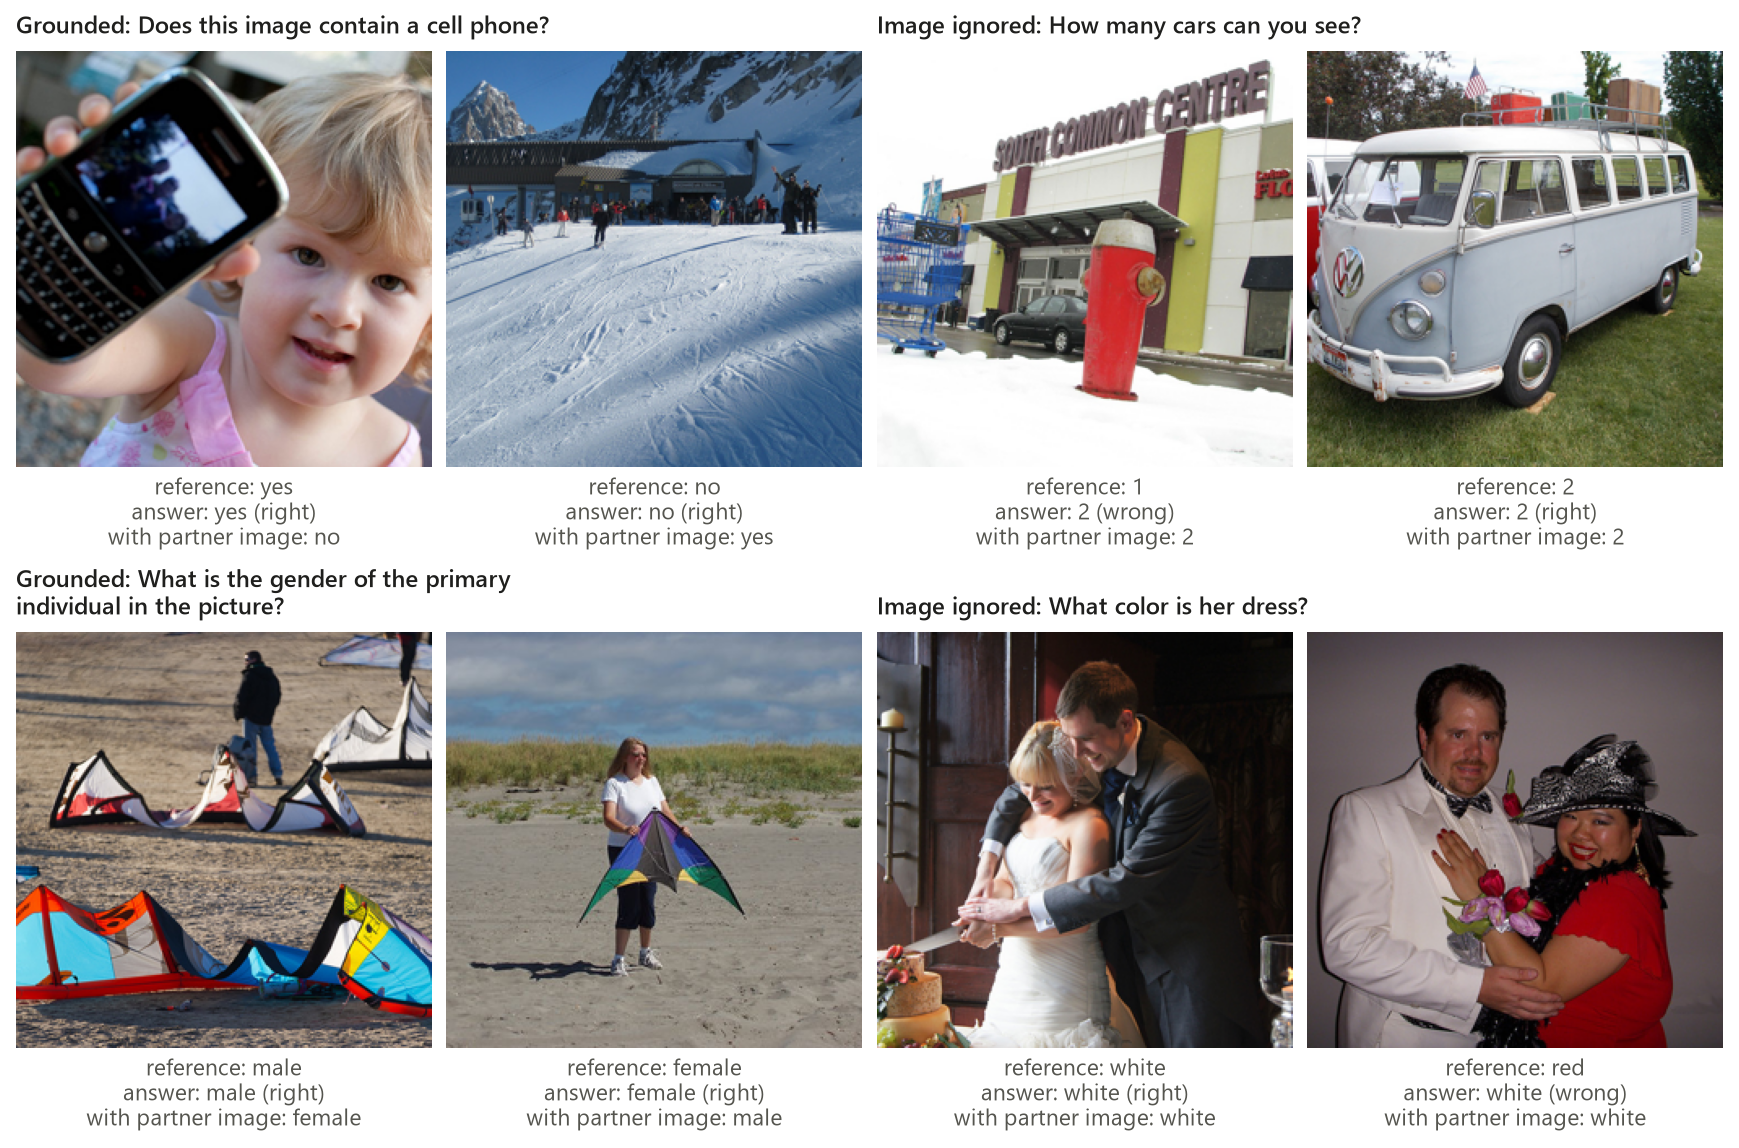
\includegraphics[width=0.8\linewidth]{figures/t2_examples.png}
\caption{Task~2 complementary pairs (rule: the first pair of each outcome category per suite; shown: grounded and image-ignored). ``With partner image'': answer to this image's question when the partner is shown. Presence and gender answers swap with the image; the car count and dress colour do not. All 28 rule-selected examples are in \texttt{results/task2/qualitative\_run196.md}.}
\label{fig:t2ex}
\end{figure}

\textbf{Measuring image use: likelihood overstates grounding.} The three measures agree in direction but not in strictness. Reference likelihood shows image use everywhere: the correct image makes the VQAv2 reference more likely than the swap (NLL advantage 0.91), even for yes/no (0.82 against 1.19). Generated accuracy shows it less, and pair accuracy least, since only 19.8\% of VQAv2 pairs are right for both images. A model can therefore prefer the right answer in likelihood while still generating the prior answer. The qualitative pairs agree (Figure~\ref{fig:t2ex}): 30 of 32 presence and 14 of 32 counting pairs are fully grounded, while 26 yes/no and 15 ``other'' VQAv2 pairs get one answer for both images, such as ``white'' for a white and a red dress. These conclusions rest on 64 and 96 test pairs, and the grounding labels inherit COCO's missing or ambiguous annotations, which our area and crowd filters reduce but cannot remove.

\begin{table}[t]
\centering
\caption{Task~2 resources for the 196-token run and the optional 49-token run ($2{\times}2$-averaged grid; same seed, data and budgets). Minutes and peak GPU memory per stage. Trainable: connector 1.84M plus LoRA 4.59M from Stage~2.}
\label{tab:t2-res}
\small
\setlength{\tabcolsep}{4pt}
\begin{tabular}{lccc}
\toprule
 & Trainable & 196 tokens & 49 tokens\\
\midrule
Feature caching, 9,270 images & -- & \multicolumn{2}{c}{3.7 min, 0.49 GB; 2.8 GB cache (shared)}\\
Stage 1 (minutes, peak GB) & 1.84M & 49.5, 1.66 & 22.2, 1.58\\
Stage 2 & 6.42M & 39.2, 1.68 & 23.9, 1.57\\
Stage 3 & 6.42M & 19.4, 1.68 & 11.9, 1.54\\
Training total; generation & & 1.80 h; 0.038 s/ans., 2.06 GB & 0.97 h; 0.025 s/ans., 1.54 GB\\
Grounding / VQAv2 (pair acc.) & & 80.5 (68.8) / 53.7 (19.8) & 77.3 (64.1) / 53.5 (22.9)\\
\bottomrule
\end{tabular}
\end{table}

\textbf{Capabilities and cost.} The VLM reliably detects trained object categories, counts small numbers with off-by-one errors, and falls back on priors for natural yes/no and attribute questions. It is also cheap: 3.7 minutes of feature caching, then 1.80 hours of training under 1.7 GB peak memory, and 0.04 s per answer (Table~\ref{tab:t2-res}). With 49 visual tokens, training takes half as long and generation a third less time, and both accuracies fall inside the 196-token intervals, so the $14\times14$ grid is not the bottleneck at this scale.

% ====================================================================================
\section{Task 3: Sampling, selection and adaptive inference}

\textbf{Setup.} We use the supplied 32 rollouts per question from Qwen2.5-3B-Instruct~\cite{qwen25} on 1,000 MATH and Qwen2.5-VL-3B-Instruct~\cite{qwen25vl} on 1,000 MathVista testmini questions, split 200/800 into development and held-out questions, with ten saved orders per question (results averaged over orders, then questions). Answers are grouped without gold labels (math-verify 0.9.0~\cite{mathverify} for MATH; type, choice and precision rules for MathVista); missing answers form one \texttt{NO\_ANSWER} group, which is always wrong but is kept in voting and in the cost. We compare FirstAns, self-consistency~\cite{wang2023selfconsistency}, highest mean log-probability, highest self-certainty~\cite{kang2025selfcertainty} and rank-weighted consensus (RWC), and for MathVista also vision-only and VisConf~\cite{usman2026visconf}, recalibrated on each revealed candidate set. Cost is the generated tokens of every candidate consumed. A live run compares three strategies on 50 held-out MATH questions under a 3,072-token output allowance, and adaptive stopping~\cite{aggarwal2023adaptive} is simulated over the saved orders.

\begin{figure}[t]
\centering
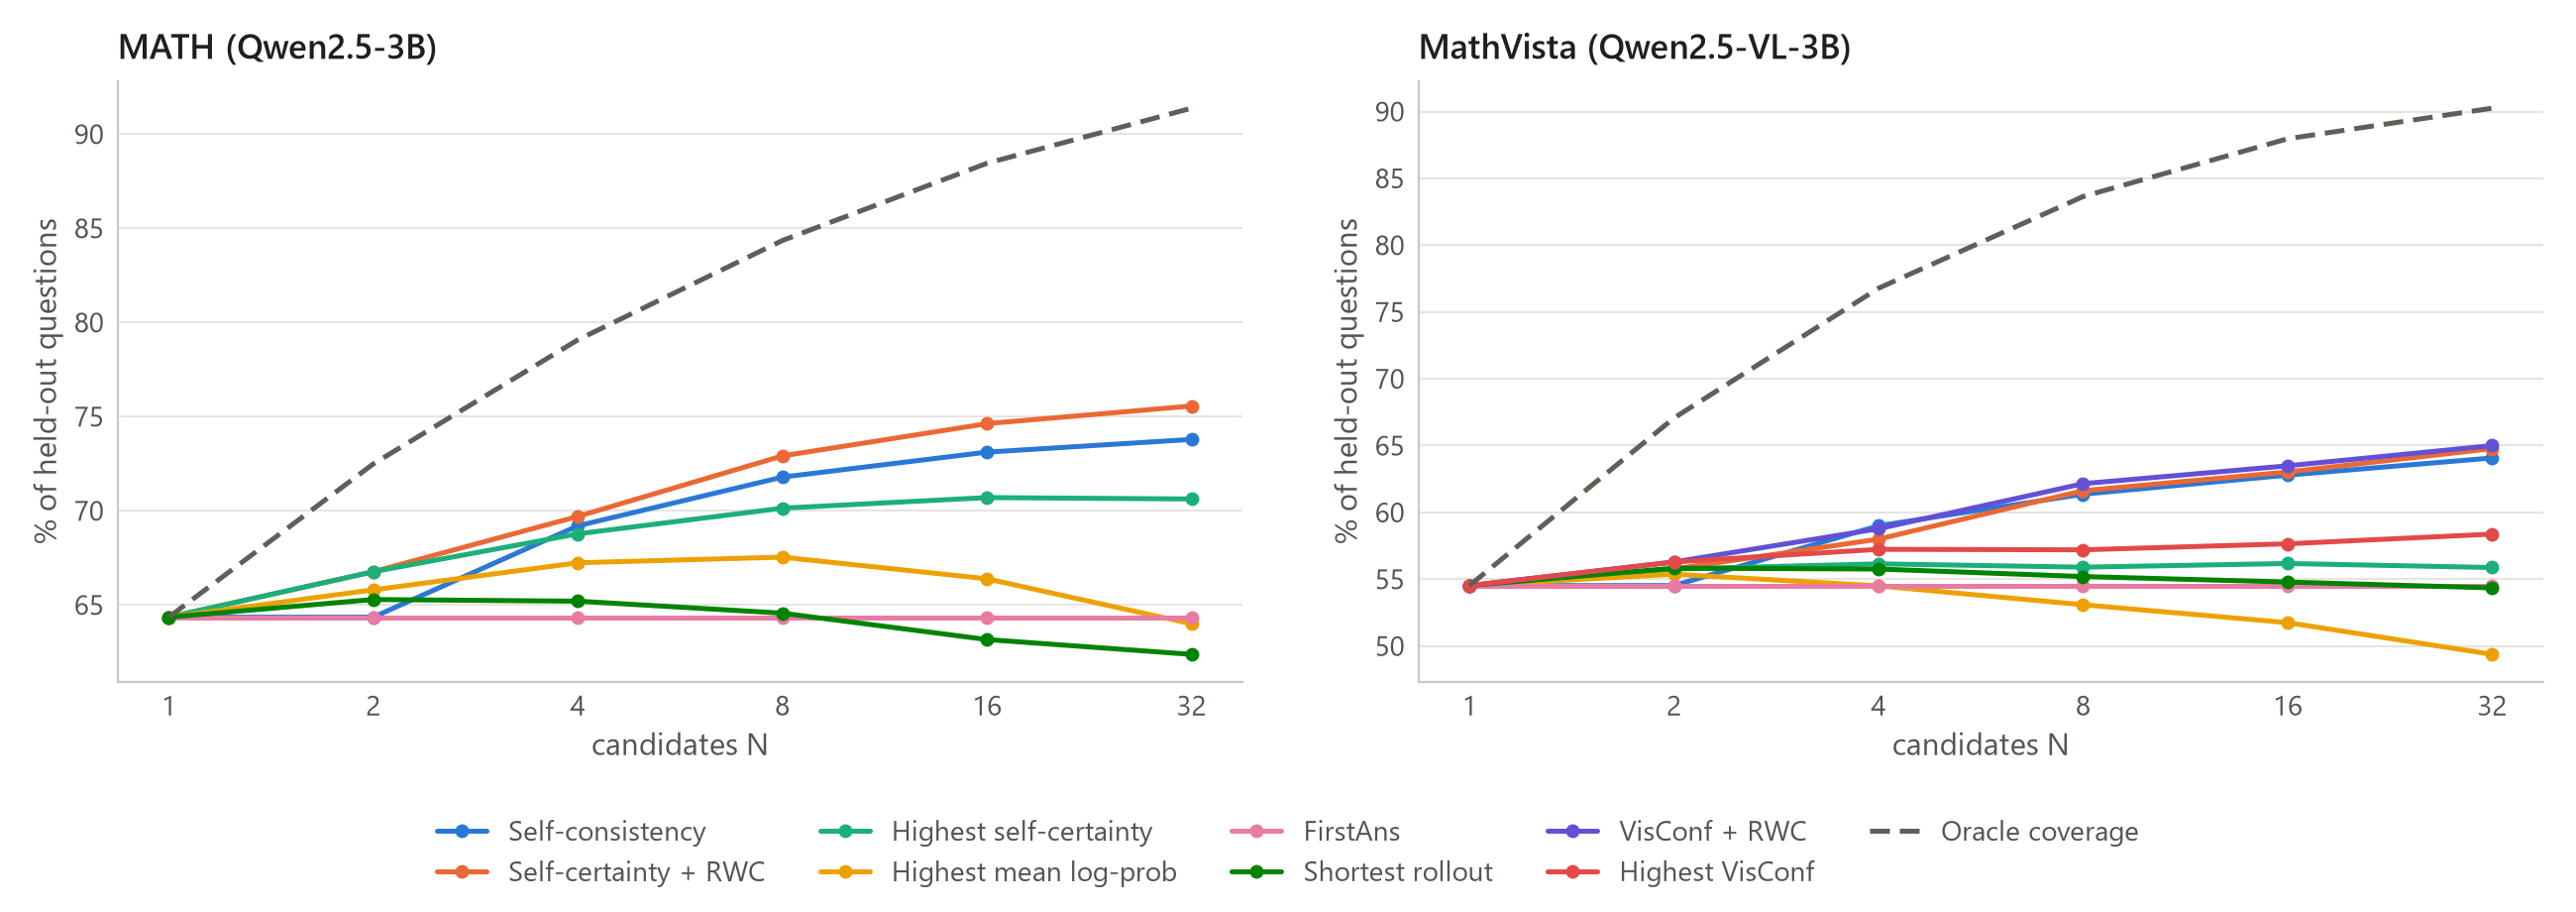
\includegraphics[width=\linewidth]{figures/t3_accuracy_coverage.png}
\caption{Task~3 held-out accuracy and oracle coverage (a correct candidate among the first $N$) against the number of candidates, averaged over ten orders. The gap between the dashed oracle curve and the best selector is the selection failure.}
\label{fig:t3}
\end{figure}

\begin{table}[t]
\centering
\caption{Task~3 held-out accuracy (\%) at $N{=}8$ and $N{=}32$, with the $N{=}32$ failure decomposition (Sel.: a correct candidate existed but was not chosen; Samp.: none existed) and mean generated tokens per question.}
\label{tab:t3}
\small
\setlength{\tabcolsep}{4pt}
\begin{tabular}{lcccc|cccc}
\toprule
 & \multicolumn{4}{c|}{MATH (Qwen2.5-3B)} & \multicolumn{4}{c}{MathVista (Qwen2.5-VL-3B)}\\
Method & $N{=}8$ & $N{=}32$ & Sel. & Samp. & $N{=}8$ & $N{=}32$ & Sel. & Samp.\\
\midrule
FirstAns & 64.3 & 64.3 & 27.0 & 8.6 & 54.5 & 54.5 & 35.7 & 9.8\\
Shortest rollout & 64.6 & 62.4 & 29.0 & 8.6 & 55.2 & 54.4 & 35.9 & 9.8\\
Highest mean log-prob & 67.5 & 64.0 & 27.4 & 8.6 & 53.1 & 49.4 & 40.9 & 9.8\\
Highest self-certainty & 70.1 & 70.6 & 20.8 & 8.6 & 55.9 & 55.9 & 34.4 & 9.8\\
Highest vision & -- & -- & -- & -- & 55.2 & 54.5 & 35.8 & 9.8\\
Highest VisConf & -- & -- & -- & -- & 57.2 & 58.4 & 31.9 & 9.8\\
Self-consistency & 71.8 & 73.8 & 17.6 & 8.6 & 61.4 & 64.1 & 26.2 & 9.8\\
Self-certainty + RWC & \textbf{72.9} & \textbf{75.6} & 15.8 & 8.6 & 61.6 & 64.8 & 25.5 & 9.8\\
Vision + RWC & -- & -- & -- & -- & 61.3 & 64.5 & 25.8 & 9.8\\
VisConf + RWC & -- & -- & -- & -- & \textbf{62.1} & \textbf{65.0} & 25.2 & 9.8\\
Oracle coverage & 84.3 & 91.4 & & & 83.6 & 90.2 & & \\
Tokens per question & 5,344 & 21,347 & & & 2,230 & 8,898 & & \\
\bottomrule
\end{tabular}
\end{table}

\textbf{Exploration and selection: sampling finds answers that selection loses.} Coverage rises from 64.3\% at $N{=}1$ to 91.4\% at $N{=}32$ on MATH and from 54.5\% to 90.2\% on MathVista (Figure~\ref{fig:t3}), but the best selector reaches only 75.6\% and 65.0\%. At $N{=}32$ the selection failures of the best methods (15.8\% and 25.2\%) are about twice their sampling failures (8.6\% and 9.8\%; Table~\ref{tab:t3}). Selection, not exploration, therefore limits repeated sampling, and the gap widens with compute. Extra samples mostly add alternatives rather than repeats: between $N{=}4$ and $N{=}32$ the number of distinct answer groups grows from 1.9 to 5.9 on MATH and from 2.0 to 4.8 on MathVista, so coverage keeps rising while the majority answer stays fixed~\cite{wang2023selfconsistency}.

\begin{table}[t]
\centering
\caption{Task~3 signals at $N{=}32$ on held-out questions with mixed correctness: correct-rate difference between the top and bottom quartile of each score within a question (points), and Spearman correlation $\rho$ of the score with rollout length.}
\label{tab:t3-sig}
\small
\setlength{\tabcolsep}{5pt}
\begin{tabular}{lcccccc}
\toprule
 & Length & Log-prob & Self-cert. & Vision & VisConf & Token-fused\\
\midrule
MATH quartile gap & $-7.8$ & $+13.4$ & $+20.4$ & -- & -- & --\\
MATH $\rho$ with length & 1 & $+0.25$ & $-0.19$ & -- & -- & --\\
MathVista quartile gap & $-4.5$ & $+2.6$ & $+4.6$ & $+4.4$ & $+9.1$ & $+9.0$\\
MathVista $\rho$ with length & 1 & $+0.36$ & $+0.35$ & $-0.69$ & $-0.29$ & $-0.33$\\
\bottomrule
\end{tabular}
\end{table}

\textbf{Evidence and consensus: confidence misleads alone but helps as a vote weight.} The single highest-scoring rollout is worse than self-consistency on both datasets, and mean log-probability even degrades with more candidates (MATH 67.5\% at $N{=}8$ falling to 64.0\%; MathVista 49.4\%, below FirstAns). The reason is that it rises with length (Table~\ref{tab:t3-sig}) while longer rollouts are more often wrong (909 against 534 tokens for incorrect and correct MATH rollouts); the shortest-rollout control is no better than FirstAns. Self-certainty separates correct rollouts best on MATH~\cite{kang2025selfcertainty}, and as RWC weights it beats self-consistency by 1.8 points \ci{0.7}{3.0}. On MathVista all signals are weak. VisConf is the best single score (2.5 points above self-certainty) and VisConf + RWC the best method, but its edge over self-consistency is not significant ($+0.9$ \ci{$-$0.4}{2.4}). Vision + RWC does as well (64.5\%), and the highest vision score alone equals FirstAns (54.5\%). Within rollouts, calibrated confidence and visual engagement are negatively correlated (median $-0.21$, positive in 11\% of questions): attention to the image peaks early and decays, while confidence follows the reasoning steps (Appendix Figure~\ref{fig:traj}). Since $Z^{\text{token}}-Z=\mathrm{Cov}_t(c,v)<0$ (mean $-0.0022$), token-wise fusion is no better under either rule (57.1\% against 58.4\% for highest-score, 64.5\% against 65.0\% for RWC). These signals measure agreement and confidence, not correctness or causal grounding.

\begin{table}[t]
\centering
\caption{Task~3 live MATH strategies on 50 held-out questions (3,072-token output allowance; the shared initial response is charged to both parallel sampling and refinement). Truncated: any call hit its cap. Transitions are relative to the shared initial answer. Peak GPU memory 6.6 GB.}
\label{tab:live}
\small
\setlength{\tabcolsep}{2.8pt}
\begin{tabular}{lccccccc}
\toprule
Strategy & Acc. & Input tok. & Output tok. & Seconds & Truncated & Extracted & W$\to$C / C$\to$W\\
\midrule
Single ($1\times3{,}072$) & 62 & 108 & 760 & 41.5 & 4\% & 96\% & --\\
Parallel ($3\times1{,}024$, vote) & 54 & 325 & 1,857 & 100.4 & 26\% & 78\% & --\\
Refinement ($1{,}024+2{,}048$) & 62 & 890 & 1,217 & 66.3 & 20\% & 100\% & 3 / 0\\
\bottomrule
\end{tabular}
\end{table}

\textbf{Breadth and refinement: short budgets, not breadth, limit parallel sampling.} One 3,072-token response and refinement both reach 62\%, while three 1,024-token samples with voting reach 54\% (Table~\ref{tab:live}). Parallel sampling is limited by its short cap, since 16.7\% of its calls hit 1,024 tokens without producing an answer, against 4\% for the single response. Refinement~\cite{madaan2023selfrefine} raises the initial accuracy from 56\% to 62\%, with three wrong-to-correct and no correct-to-wrong transitions. It changes 20\% of the answers and always ends with an extractable answer, but it costs the most input tokens (890, because the revision prompt contains the initial response) and 66 s against 42 s. No paired difference is significant with 50 questions (parallel minus single $-8$ \ci{$-$20}{+6}).

\begin{table}[t]
\centering
\caption{Task~3 adaptive stopping on held-out questions with development-selected settings (lowest cost within one point of fixed-32 on development). Both controllers return the current self-consistency answer; the quality controller uses self-certainty (MATH) or VisConf (MathVista). Wrong early: stops before 32 with a wrong answer, of 8,000 question-orders; in brackets, those fixed-32 voting would have answered correctly.}
\label{tab:adapt}
\small
\setlength{\tabcolsep}{3pt}
\begin{tabular}{llcccccc}
\toprule
 & Policy ($\tau$, $\gamma$) & Acc. & $\Delta$ fixed-32 & Tokens & Rollouts & Stops 4/8/16/32 (\%) & Wrong early\\
\midrule
\multirow{3}{*}{MATH} & Agreement (0.625) & 73.6 & $-0.15$ & 10,140 & 11.8 & 66 / 6 / 1 / 27 & 660 (51)\\
 & Quality (0.5, 0) & 73.2 & $-0.60$ & 7,658 & 9.0 & 76 / 6 / 1 / 16 & 1,153 (131)\\
 & Fixed 4 / 8 / 16 & \multicolumn{5}{l}{69.2 / 71.8 / 73.1\% at 2,680 / 5,344 / 10,678 tokens} & \\
\midrule
\multirow{3}{*}{MathVista} & Agreement (0.5) & 63.1 & $-0.95$ & 3,029 & 8.9 & 75 / 8 / 2 / 15 & 1,930 (333)\\
 & Quality (0.5, 0) & 63.6 & $-0.50$ & 3,384 & 10.0 & 68 / 10 / 3 / 19 & 1,709 (262)\\
 & Fixed 4 / 8 / 16 & \multicolumn{5}{l}{59.0 / 61.4 / 62.8\% at 1,112 / 2,230 / 4,462 tokens} & \\
\bottomrule
\end{tabular}
\end{table}

\textbf{Adaptive allocation: early agreement is a cheap stopping signal.} The selected policies stop after four candidates in 66--76\% of held-out question-orders and nearly match fixed-32 self-consistency at a third of the cost (Table~\ref{tab:adapt}). On MATH the quality controller loses 0.60 points \ci{$-$1.20}{$-$0.01} with 64\% fewer tokens, and the agreement controller 0.15 (not significant) with 53\% fewer; on MathVista both lose 0.5--1.0 points (not significant) with 62--66\% fewer. Another rollout is useful mainly when the early candidates disagree. Retrospectively, the MATH agreement controller stops at four on every question whose pool is all correct, but on only 21\% of those where at most half is correct (24 rollouts on average), and it stops at four 97\% of the time when the leading group holds over 75\% of the pool.

\begin{table}[t]
\centering
\caption{Task~3 rule-selected cases (held-out questions in split order, saved order 0; first case of each type).}
\label{tab:t3ex}
\scriptsize
\begin{tabular}{>{\raggedright\arraybackslash}p{0.15\linewidth}>{\raggedright\arraybackslash}p{0.28\linewidth}>{\raggedright\arraybackslash}p{0.47\linewidth}}
\toprule
Case & Question & What happened\\
\midrule
Tie broken by weights & MATH \texttt{test:2460}, sum of two smallest $N$ (gold 154) & Votes split 154 $\times$11 vs.\ 58 $\times$11; self-consistency picks 58 by tie-break, self-certainty + RWC picks 154\\
Weights override majority & MATH \texttt{test:2198}, $g(f(x))$ (gold 11) & Gold leads with only 5 of 32 votes; RWC moves to 14 (4 votes)\\
Premature stop & MATH \texttt{test:1803}, $\sin X$ (gold 3/5) & Quality controller stops at 8 with 4/5 leading 6 to 2; the full pool favours 3/5, 16 to 15\\
Revision W$\to$C & MATH \texttt{test:196}, lattice points (gold 81) & Initial response cut off mid-count with no answer; the revision completes the count: 81\\
\bottomrule
\end{tabular}
\end{table}

\textbf{Compute and reliability.} At similar cost the adaptive policies beat fixed budgets (MATH: 73.2\% at 7,658 tokens against 71.8\% for $N{=}8$ at 5,344 and 73.1\% for $N{=}16$ at 10,678; Appendix Figure~\ref{fig:t3cost}), so consensus with a quality weight and early stopping gives the best accuracy--cost trade-off. Its failures are informative (Table~\ref{tab:t3ex}). Early stops go wrong when the first candidates agree on a wrong answer, which is common on MathVista: 333 early stops were wrong although fixed-32 voting was right. Agreement measures consistency, not correctness, and the remaining selection gap shows that internal signals cannot yet recognize correct minority answers. Token counts exclude prefill, attention collection and scoring, and the two datasets differ in model and question type, so they do not isolate the effect of vision.

\FloatBarrier
% ====================================================================================
\section{Conclusion}
In all three tasks the headline gains came partly from answer format, language priors or agreement rather than from the intended capability. Only controlled comparisons with matching diagnostics, namely rescoring, complementary pairs and oracle coverage, made those gains interpretable. Several limitations remain. Task~1 used one seed per method, so GSM8K differences under about 1.5 points are noise, its rescoring is a heuristic, and its recovery checkpoints were deleted after training. Task~2 labels depend on our area and crowd thresholds, and its test suites are small. Task~3 ran only 50 live questions and reports offline token costs. Next steps are more seeds, a format-robust GSM8K extractor, VQA training that balances prior-predictable questions, and selectors that can recognize correct minority answers.

\bibliographystyle{plain}
\bibliography{refs}

% ====================================================================================
\newpage
\appendix
\counterwithin{table}{section}
\counterwithin{figure}{section}

\section{Experimental details and deviations}\label{app:details}

\begin{table}[h]
\centering
\caption{Settings for all three tasks.}
\label{tab:settings}
\small
\begin{tabular}{p{0.16\linewidth}p{0.78\linewidth}}
\toprule
Task 1 model & \texttt{Qwen/Qwen3-0.6B} (revision \texttt{c1899de}), \texttt{enable\_thinking=False} throughout\\
Task 1 data & First 40,000 eligible MetaMathQA examples in source order (excluded: empty fields, over 2,048 tokens, or query matching a GSM8K test question); not shuffled or truncated; loss on response and end-of-turn tokens, normalized over valid tokens in the effective batch\\
Task 1 training & 1,250 AdamW updates (betas 0.9/0.999, $\epsilon=10^{-8}$), microbatch 2 $\times$ accumulation 16, weight decay 0.01 (not on biases or 1-D parameters), cosine decay with 38 warm-up updates, clipping 1.0 after unscaling, FP16 autocast with dynamic loss scaling, FP32 optimizer states, gradient checkpointing. Full FT and L2-SP: FP32 master weights, peak LR $2\times10^{-5}$, L2-SP $\lambda=10^{-3}$ over all unique parameters (tied counted once). LoRA-4 ($\alpha{=}8$), LoRA-16 ($\alpha{=}32$), OPLoRA-16 ($k{=}128$, bases computed once in FP32): dropout 0.05, random $A$, zero $B$, no biases, all seven projections of every layer, frozen FP16 backbone, FP32 adapters, peak LR $2\times10^{-4}$\\
Task 1 evaluation & lm-evaluation-harness 0.4.13 (HF backend, FP16, dropout off). GSM8K \texttt{gsm8k\_cot}, \texttt{num\_fewshot=0}, chat template, greedy, 1,024 new tokens, stock stop rules and filters, batch 32; HellaSwag, BoolQ, ARC-Easy with stock prompts, no chat template, full splits. Probes: 32 GSM8K test and 32 HellaSwag validation items sampled with seed 6304 before results; diagnostics in FP32. Qualitative: all 24 prompts, greedy, 512 tokens\\
Task 2 model & \texttt{google/siglip-base-patch16-224} (frozen; features cached in FP16), connector Linear 768$\to$1024, GELU, Linear 1024$\to$1024, Qwen3-0.6B (frozen; LoRA from Stage~2)\\
Task 2 data & 6,000 \texttt{train2014} images $\times$ 3 captions, 96 development captions, grounding pools from training images (dev 24 pairs, test 64), VQAv2 pairs 1,536 / 32 / 96 (640/256/640, 12/8/12, 36/24/36 yes/no/number/other), kept only when the two normalized consensus answers differ and at least 8 of 10 annotators agree on each image, with an original consensus answer string as the training target and all ten answers retained for scoring; splits image-disjoint (asserted); 72,000 example presentations over 4,500 updates\\
Task 2 training & Microbatch 8 $\times$ accumulation 2, AdamW, weight decay 0.01, clipping 1.0, per-stage 5\% warm-up then cosine to 10\% of peak; caps: question 80, caption 64, answer 16 tokens; Stage 1/2/3: 2,250/1,500/750 updates, connector LR $10^{-3}$/$10^{-4}$/$5\times10^{-5}$, LoRA ($r{=}16$, $\alpha{=}32$, dropout 0.05, q/k/v/o) LR $2\times10^{-5}$/$10^{-5}$; example-weighted loss; development evaluation at 0, every 500, and 2,250/3,750/4,500; checkpoints every 250 updates\\
Task 2 evaluation & Greedy, 16 tokens, batch 8; official VQA answer normalization~\cite{antol2015vqa}; mismatched mapping fixed before generation from another pair in the same suite, excluding both images of the original pair, and reused across comparisons; no-image inputs rebuild masks and positions; 4,000 pair bootstrap resamples\\
Task 3 data & Supplied 32 rollouts per question (temperature 0.7, top-$p$ 0.8, top-$k$ 20, 2,048-token cap); question IDs sorted and permuted with \texttt{default\_rng(6304)}; first 200 development, remaining 800 held-out; first 50 held-out MATH questions for the live run\\
Task 3 selection & Budgets $N\in\{1,2,4,8,16,32\}$; ties broken by earliest supporting rollout; RWC weights $w_i=(N-r_i)/(N-1)$ with average ranks; VisConf calibrated with linear-interpolation 5th/95th percentiles of the current candidate set; adaptive grid $\tau\in\{0.5,0.625,0.75,0.875,1.0\}$, $\gamma\in\{0,0.1,0.25,0.5\}$ with the always-32 fallback, checks after 4, 8, 16, else 32, ties broken by higher development accuracy then smaller $\tau$ and $\gamma$; scores, VisConf calibration and ranks recomputed from revealed candidates only, and no gold answer or unrevealed candidate enters any selection or stopping rule; 1,000 paired question bootstrap resamples\\
Task 3 live & Qwen2.5-3B-Instruct (README revision), FP16, batch 1, temperature 0.7, top-$p$ 0.8, top-$k$ 20, repetition penalty 1.0, independent seeds per call, native chat template and prescribed prompts, last boxed answer by balanced braces\\
\bottomrule
\end{tabular}
\end{table}

\textbf{Deviations.} \emph{Task~1:} recovery checkpoints (optimizer, scheduler, scaler, RNG and data position at updates 312, 625, 937 and 1,250) were written and then deleted after training to fit Kaggle's 20 GB output limit. GSM8K was first run at batch size 1 for four conditions; we reran those at batch 32 so all seven match (accuracy changed by at most 0.3 points; both runs are kept). No update was skipped by the loss scaler, and the first update uses learning rate 0 under the standard warm-up convention. \emph{Task~2:} presence ``yes'' images need a non-crowd instance covering at least 2\% of the image and ``no'' images no instance of the category; counting uses counts 1--4 with every instance covering at least 1\% and no crowd annotation. The optimizer is rebuilt at each stage boundary with that stage's rates. Before training we checked feature shapes, frozen parameter sets, gradient flow to the connector and split isolation. The loss scaler skipped six of the first 16 updates (initial overflows) and none afterwards. \emph{Task~3:} one MATH question (\texttt{test:4928}) exceeded math-verify's 120-second limit and was grouped by exact string match.

\section{Task 1 supplementary results}\label{app:t1}
\begin{figure}[h]
\centering
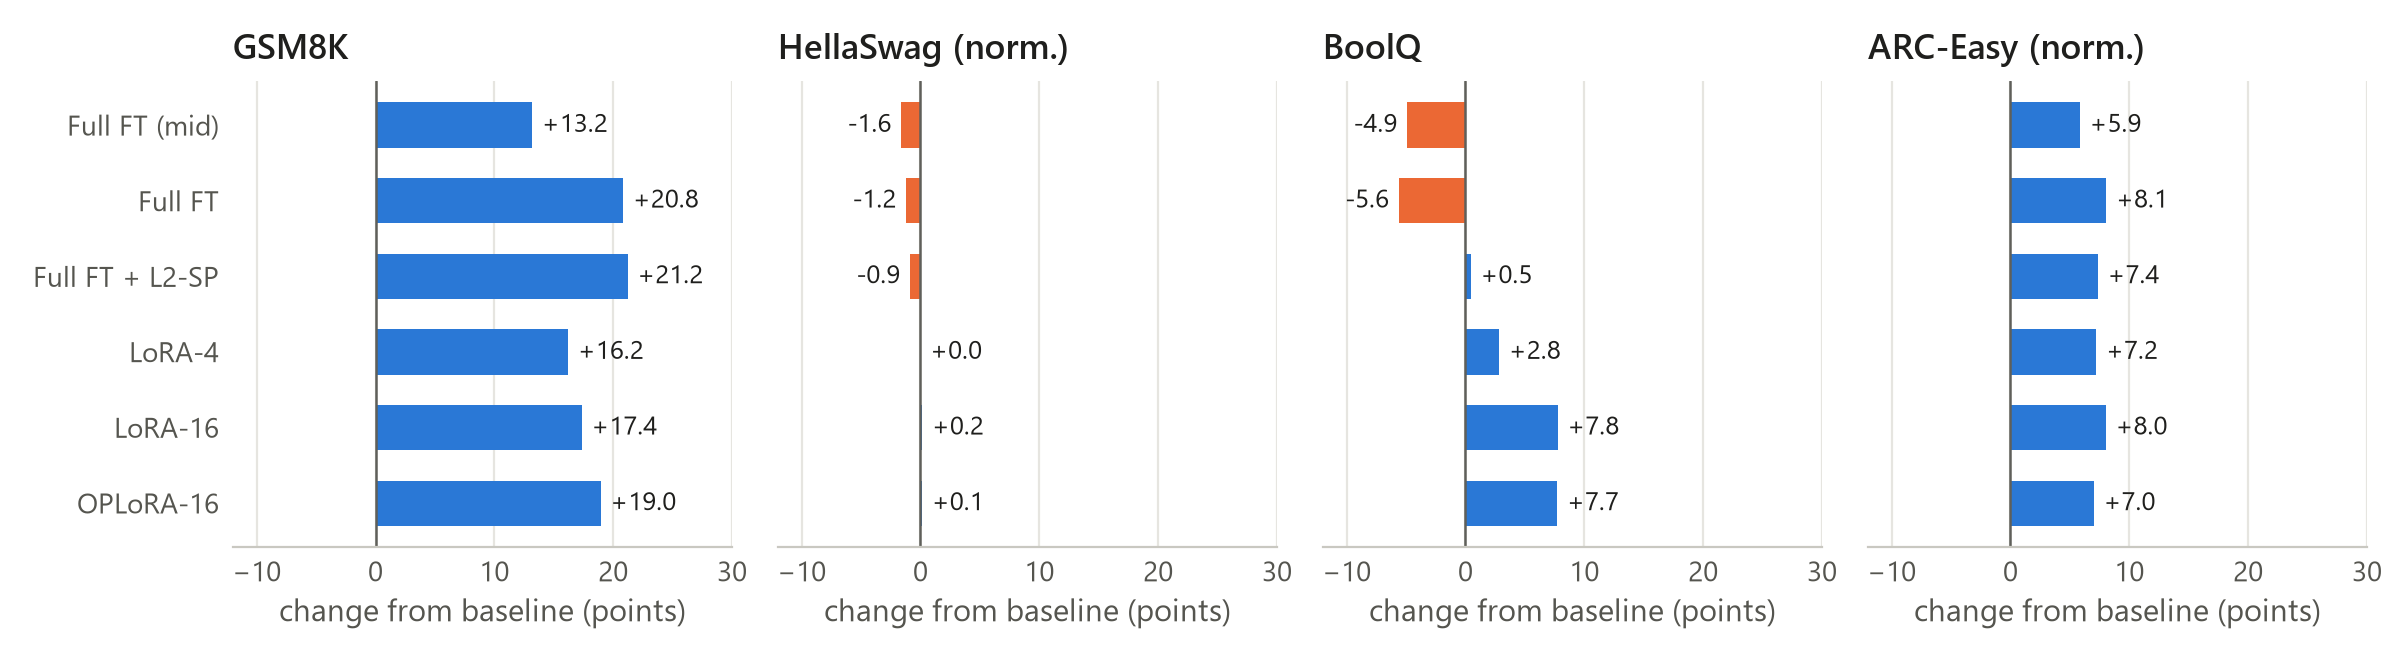
\includegraphics[width=\linewidth]{figures/t1_benchmark_changes.png}
\caption{Change from the baseline in points on the primary metric of each benchmark (stock scoring).}
\end{figure}

\section{Task 3 supplementary results}\label{app:t3}
\begin{figure}[h]
\centering
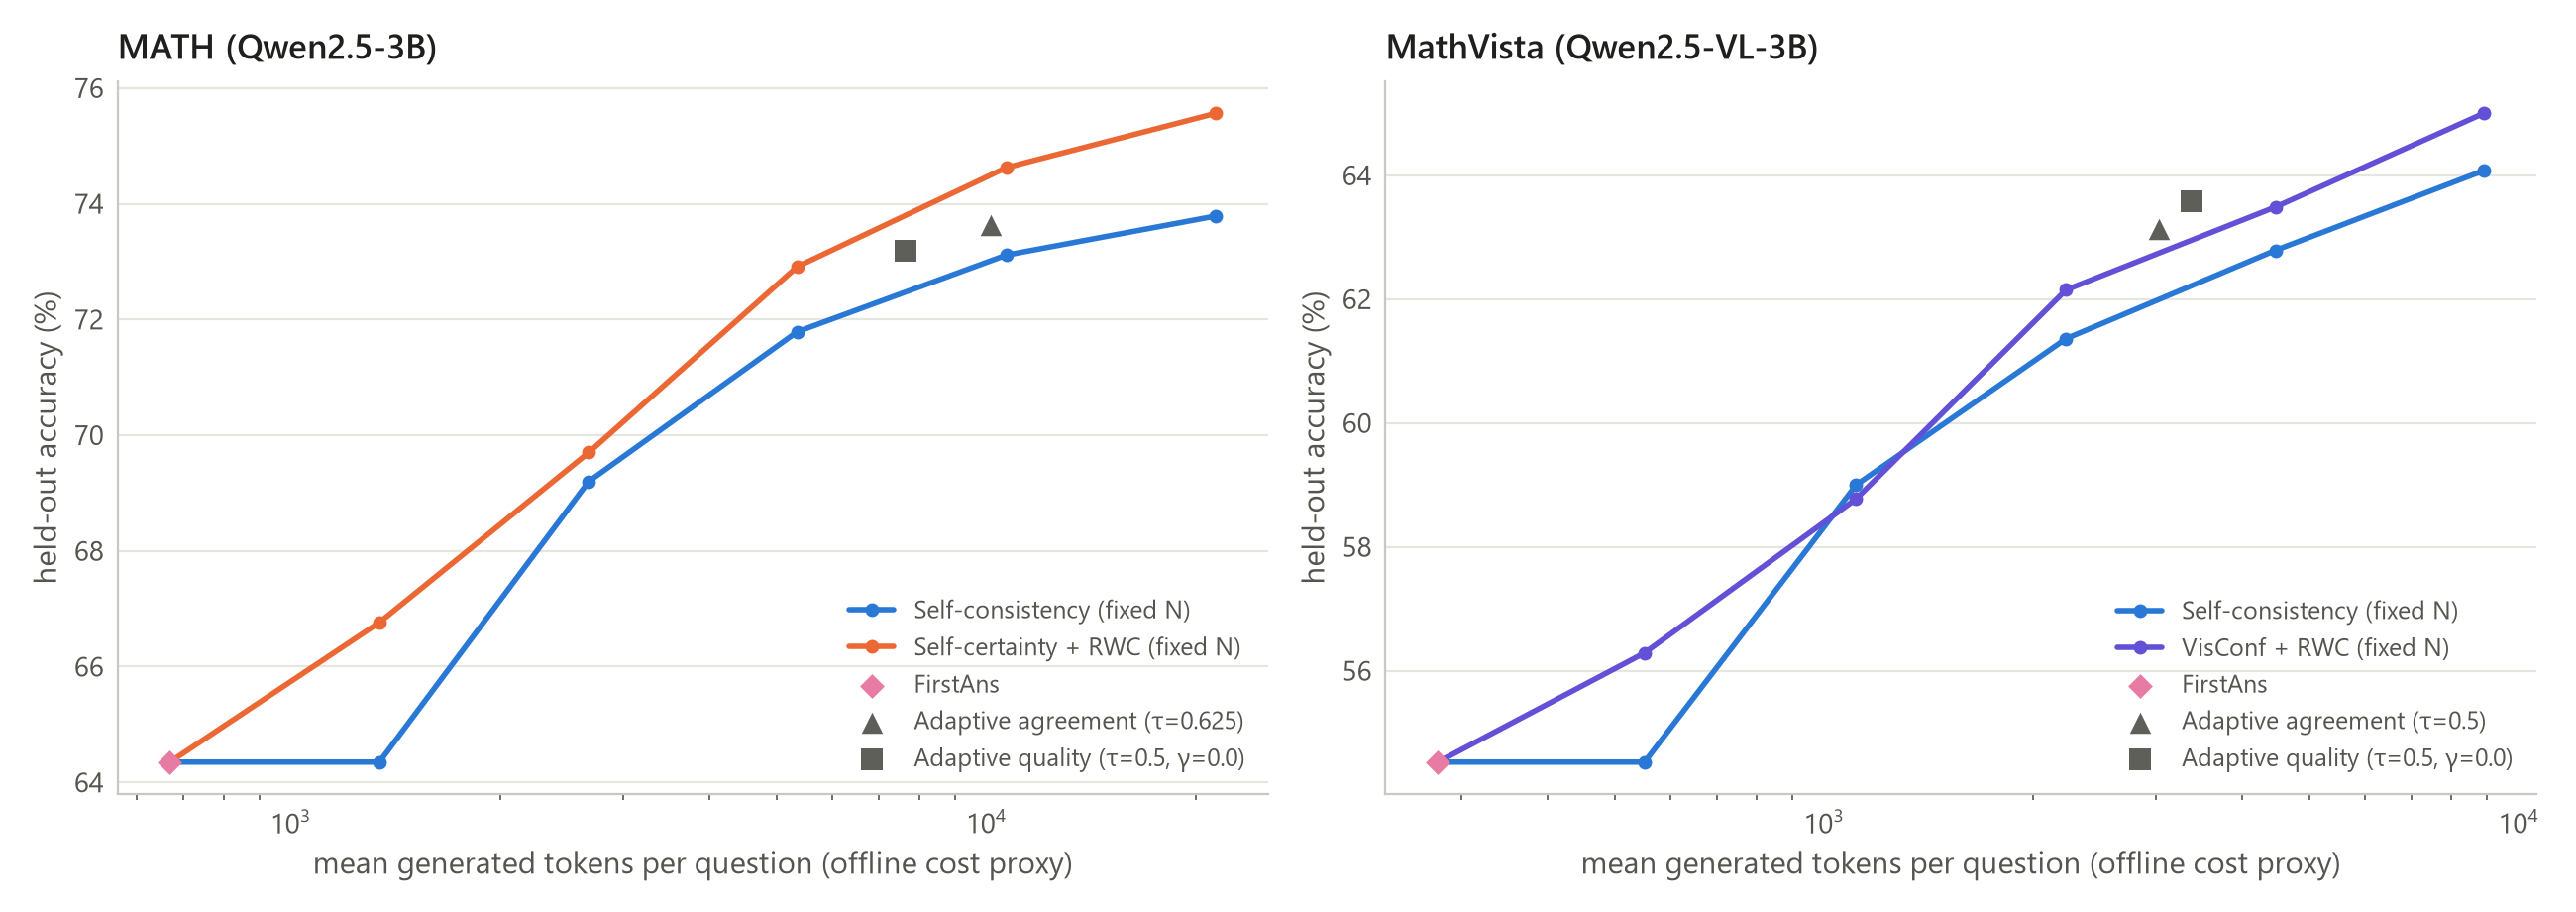
\includegraphics[width=\linewidth]{figures/t3_accuracy_vs_cost.png}
\caption{Accuracy against mean generated tokens: fixed-$N$ curves and the development-selected adaptive policies.}
\label{fig:t3cost}
\end{figure}
\begin{figure}[h]
\centering
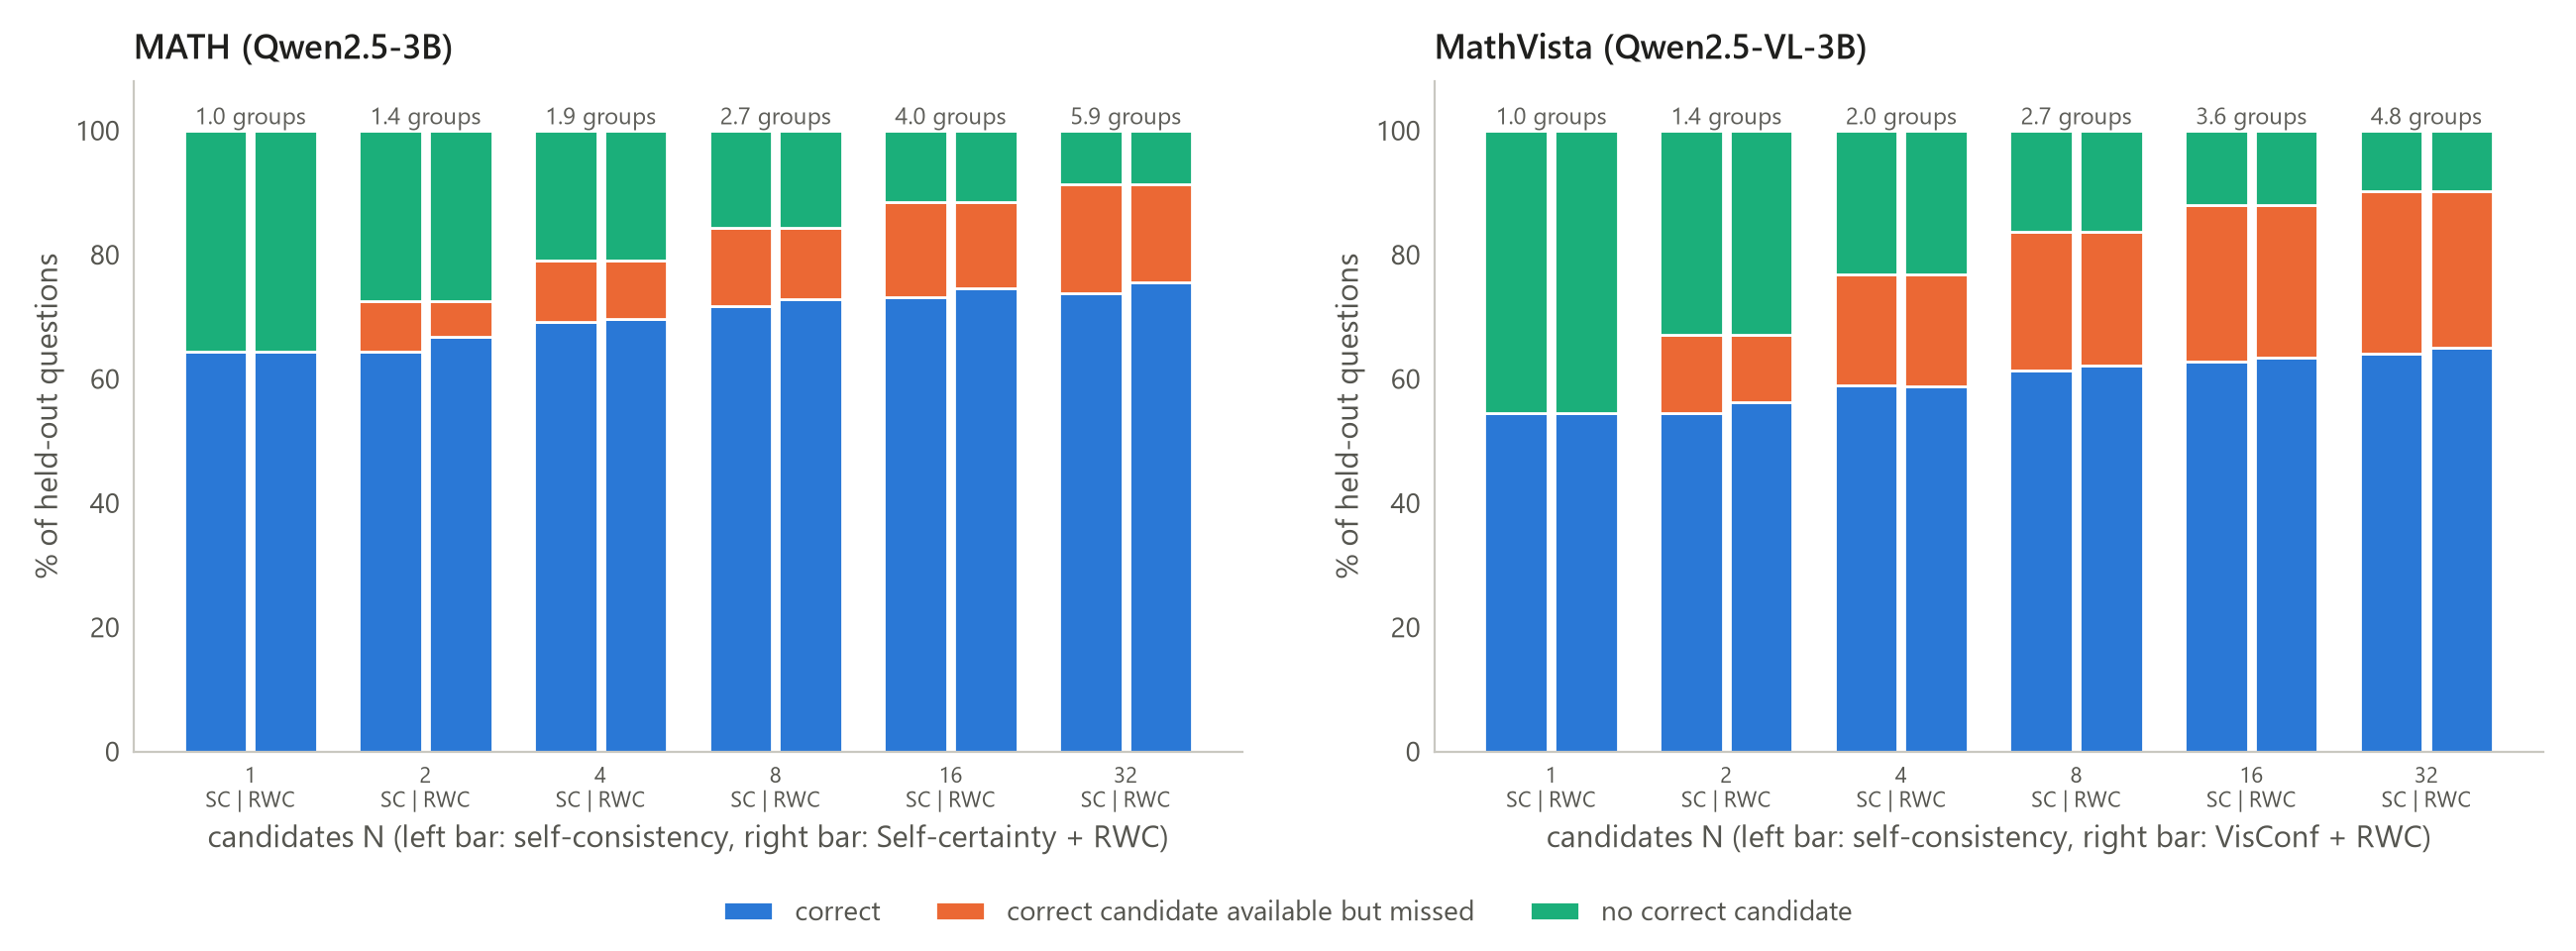
\includegraphics[width=\linewidth]{figures/t3_failure_decomposition.png}
\caption{Correct answers, selection failures (a correct candidate was available) and sampling failures (none was), with the mean number of distinct answer groups.}
\end{figure}
\begin{figure}[h]
\centering
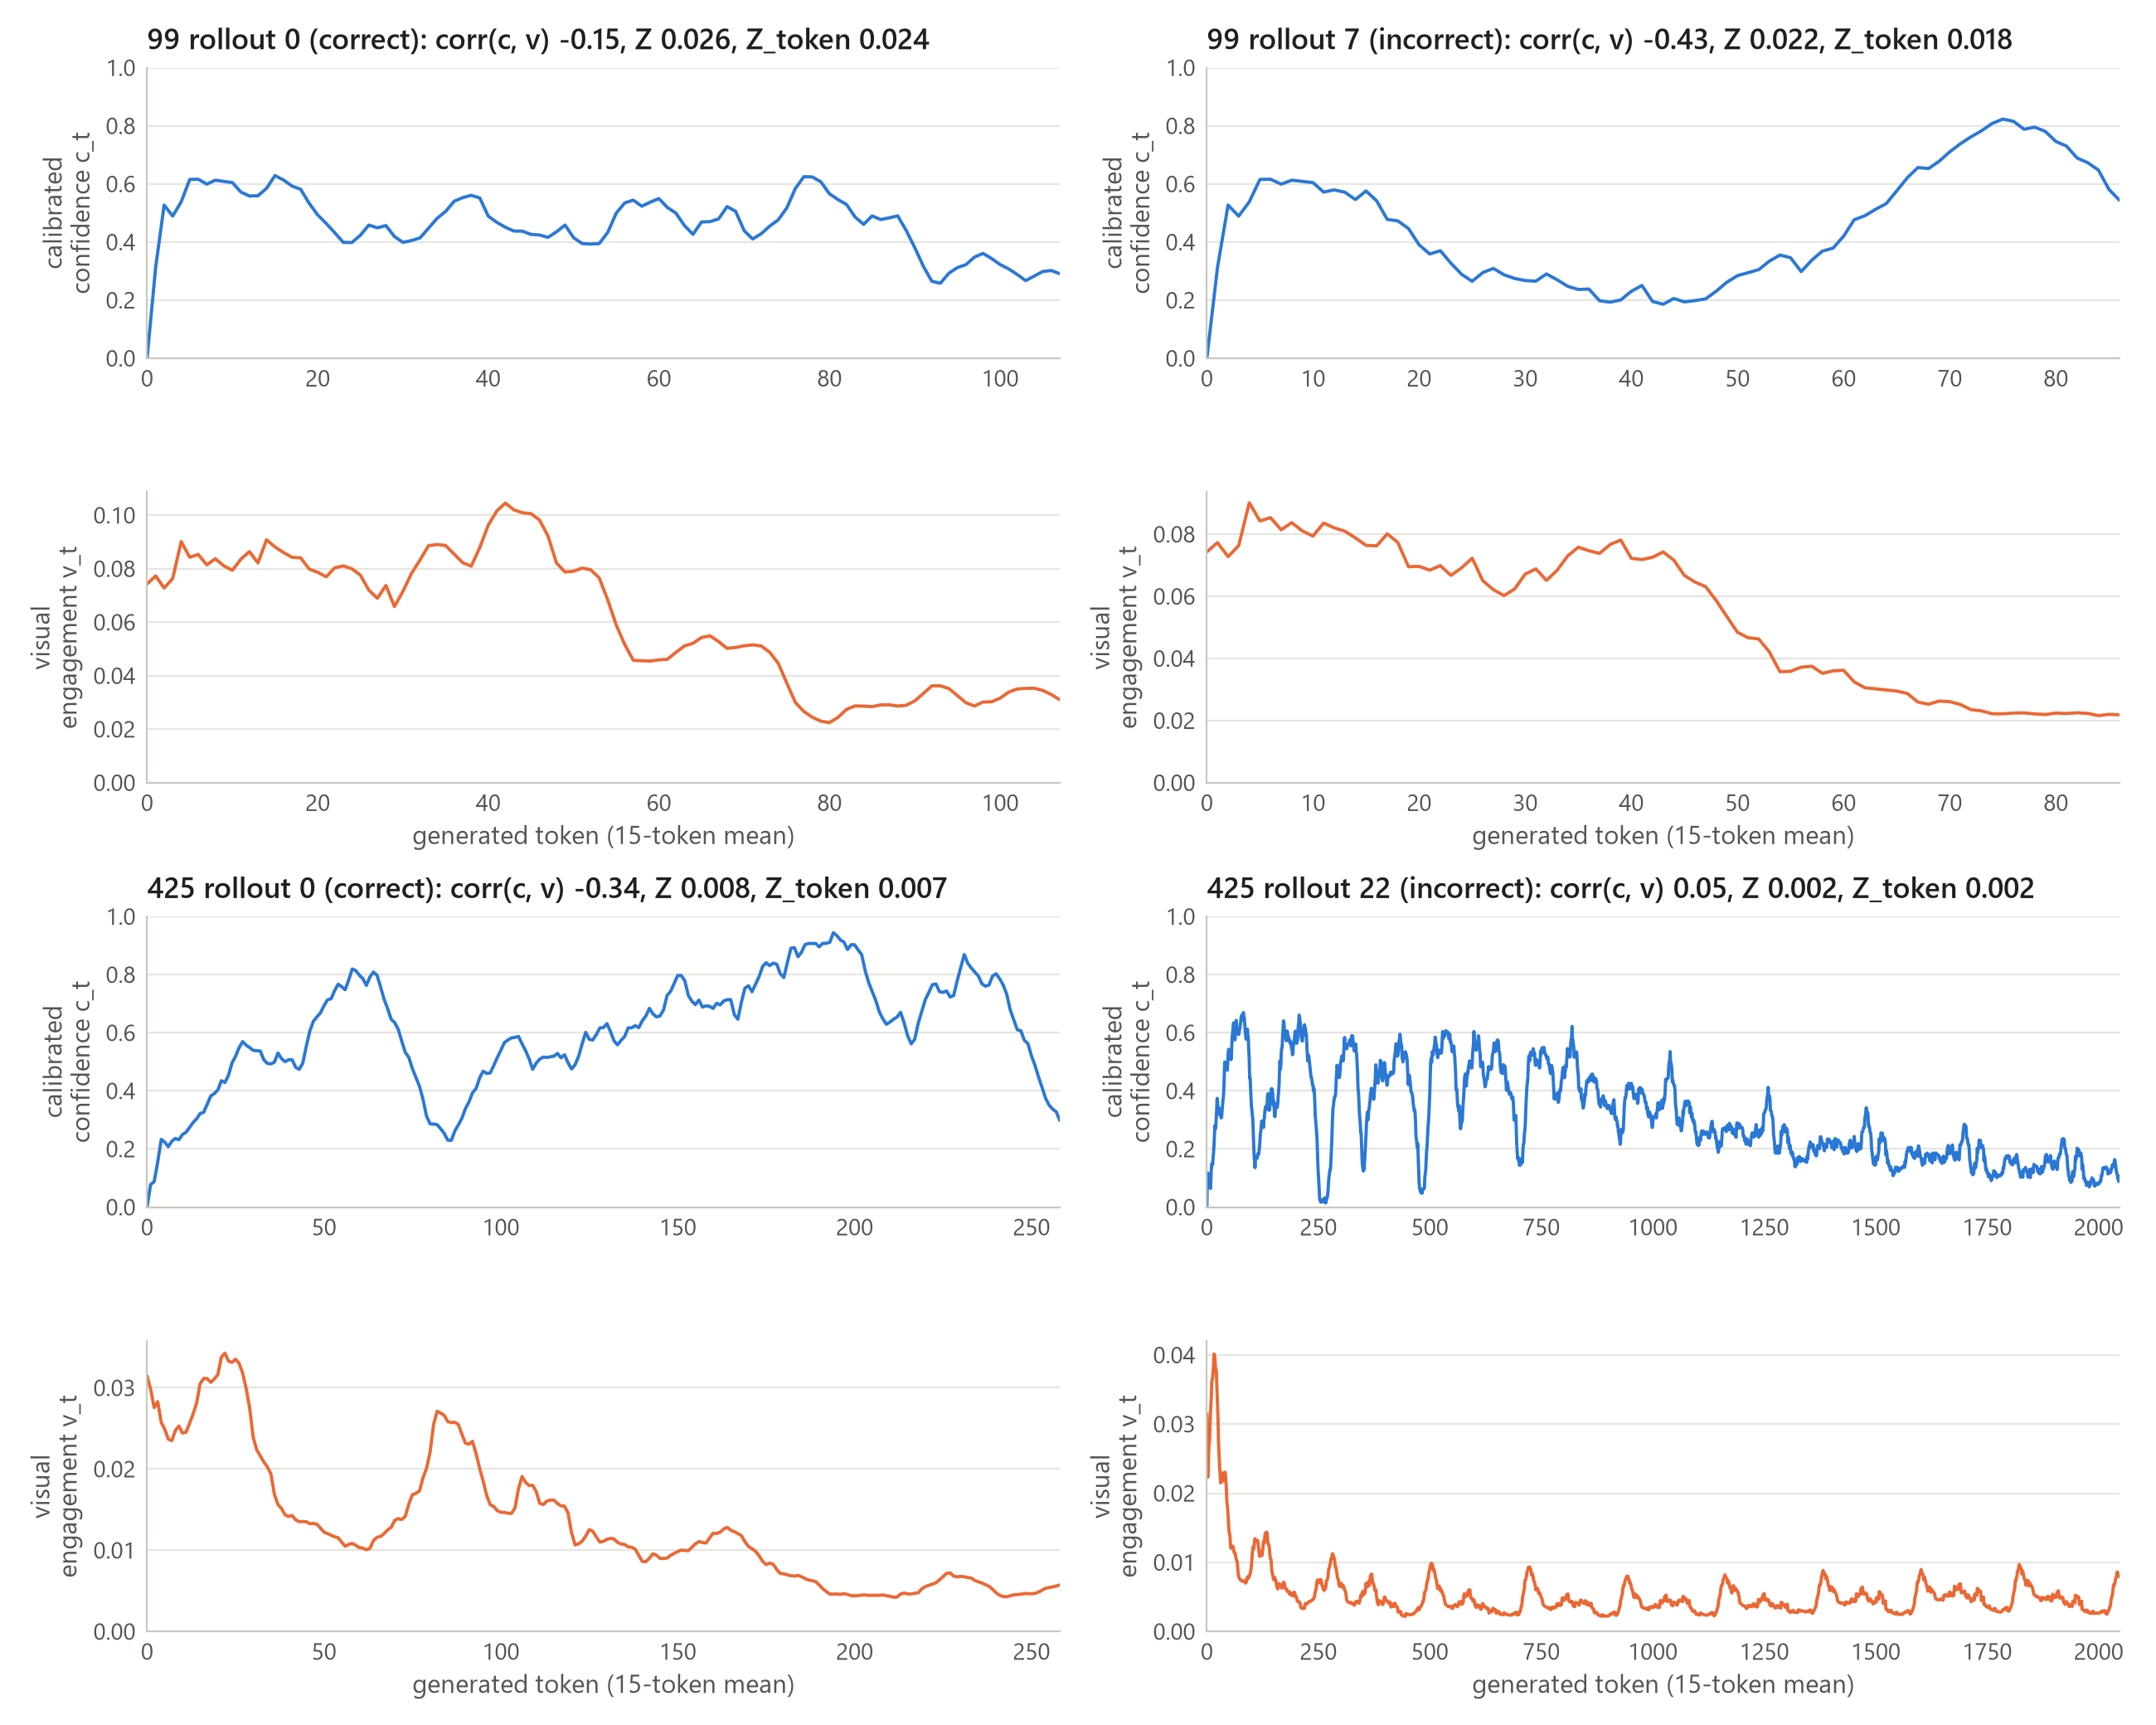
\includegraphics[width=0.9\linewidth]{figures/t3_trajectories.png}
\caption{Calibrated confidence $c_t$ and visual engagement $v_t$ along four MathVista rollouts (rule: the first two held-out questions with mixed correctness; earliest correct and earliest incorrect rollout). Visual engagement is highest at the start and decays; the incorrect rollout of question 425 runs to the 2,048-token cap with periodic confidence collapses.}
\label{fig:traj}
\end{figure}

\clearpage
\section{Additional qualitative cases}\label{app:cases}
\textbf{Task 1, template format.} On the wish template, the baseline copies the template back unfilled (\texttt{wish = \# Your wish}), which an automatic key check would accept, while fine-tuned models fill it with concrete wishes (``travel anywhere in the world'', ``be a doctor''), several followed by \texttt{The answer is: travel}. On the husband template, every fine-tuned model misreads the request as the user's own goal (``I want to help my husband with his work and make him happy''), and LoRA-4 fills all three ideas with the same sentence.

\textbf{Task 2, remaining categories.} \emph{Wrong but image-sensitive:} ``How many ties can you see?'' (references 1/2) is answered 2/1, the reverse of the references. \emph{Image ignored on yes/no:} ``Are these kitchen utensils?'' (no/yes) is answered ``yes'' for both images. Pair outcomes (grounded / ignored / wrong): presence 30/2/0; counting 14/11/7; VQAv2 yes/no 7/26/3, number 4/6/14, other 8/15/13.

\textbf{Task 3, MathVista.} On question 643 (circle geometry), self-consistency picks C (11 votes) over the gold A (10 votes), and VisConf + RWC picks A. On question 552 (``How many queries have a p-value lower than 0.50?''), self-consistency picks the gold 4 (14 votes) but VisConf + RWC picks 2 (9 votes). On question 434, the quality controller stopped after 4 candidates with C leading, although the gold A wins 17 of 32 in the full pool. In the live run, on \texttt{test:2177} the revision produced an answer where the initial response had none, but it was wrong (6 against 18).

\end{document}
